\chapter{Applications}\label{ch:appls}



In this chatper, we now apply the theoretical developments of \Cref{ch:linear_theory} and the mixture model algorithm described in \Cref{ch:gmm} to four different applications, using models constructed from observed data.
We do not investigate any of these four applications in detail; rather, the aim is to demonstrate the applicability of the theory to a range of examples.



\section{Numerical considerations}






\subsection{Numerically solving the Fokker-Planck equation}

The probability density function \(p\!\left(x,t\right)\) at any time of the solution to the SDE \cref{eqn:sde}



We solve the Fokker-Planck equation numerically using the method of lines \citep{}, which discretises the spatial variable to approximate the PDE solution with a system of ordinary differential equations.
The spatial domain is divided into a fixed number of bins


\section{The Hellinger distance}
To quantify the distance between probability distributions, we use the Hellinger distance.
The Hellinger distance is an example of an \(f\)-divergence, a broader class of measures between two probability distributions.
For two continuous probability distributions in \(\R^n\) with PDFs \(p\) and \(q\), the Hellinger distance between the two distributions is given by
\[
	D_H\!\left(p, q\right) = \sqrt{\frac12 \int_{\R^n}{\left(\sqrt{p(x)} - \sqrt{q(x)}\right)^2\dif x}} = \sqrt{1 - \int_{\R^n}{\sqrt{p(x)q(x)}\dif x}}
\]
For two discrete distributions \(\hat{P}\) and \(\hat{Q}\) defined on the same support with respective probability mass functions \(p_1, p_2, \dotsc, p_K\) and \(q_1, q_2, \dotsc, q_K\), the Hellinger distance is
\begin{equation}\label{eqn:hell_disc}
	D_H\!\left(\hat{P}, \hat{Q}\right) = \sqrt{\frac12 \sum_{i=l}^{K}\left(\sqrt{p_i} - \sqrt{q_i}\right)^2}
\end{equation}
We will use the Hellinger distance to compare three estimates of the solution to a stochastic differential equations: numerical samples from a numerical solver, analytic probability density functions from the linearised approximation and Gaussian mixture model algorithm, and a spatially discretised solution to the Fokker-Planck equation.

The state space is divided into \(K\) non-overlapping bins \(b_1, b_2, \dotsc, b_K \subset \R^n\)
Given \(N\) samples, the empirical probability corresponding to a bin is the (normalised) number of samples that fall within that bin.
With two empirical PDFs constructed over the same set of bins, we can then compute the Hellinger distance using the discrete formulation \cref{eqn:hell_disc}

The Hellinger distance is symmetric and defines a metric on the space of probability distributions.



% \subsection{The Wasserstein metric}
% To evaluate the performance of our mixture model and compare to other approaches (such as stochastic simulation), we require a measure that compares probability distributions.
% The Wasserstein distance (also known as the earth mover's distance) is one such metric between probability distributions.
% The Wasserstein \(p\)-distance, for \(p \geq 1\), is defined formally as follows.
% Let \(\mu\) and \(\nu\) denote two probability measures on \(\R^n\), each with finite \(p\)-moments.
% Then, the Wasserstein \(p\)-distance between \(\mu\) and \(\nu\) is
% \[
% 	W_p\!\left(\mu, \nu\right) = \left(\inf_{\gamma \in \Gamma\!\left(\mu, \nu\right)}\mathds{E}_{(x,y) \in \gamma}\!\left[\norm{x - y}^p\right]\right)^{1/p},
% \]
% where \(\Gamma\!(\mu, \nu)\) is the set of all couplings of \(\mu\) and \(\nu)\).
% A coupling \(\gamma\) between \(\mu\) and \(\nu\) is a probability measure on \(\R^n \times \R^n\) such that the marginals are \(\mu\) and \(\nu\), i.e.
% \begin{align*}
% 	\int_{\R^n}{\gamma(x,y)\dif y} & = \mu(x), \\
% 	\int_{\R^n}{\gamma(x,y)\dif x} & = \nu(y).
% \end{align*}
% If \(\mu\) and \(\nu\) admit the respective probability density functions \(p, q \colon \R^n \to [0,\infty)\), then the Wasserstein distance can be written as
% \[
% 	W_p\!\left(p, q\right) = \left(\inf_{\gamma \in \Gamma\!\left(p,q\right)}\int_{\R^n \times \R^n}{\norm{x - y}^p \gamma\!\left(x,y\right)\dif x\dif y}\right)^{1/p}.
% \]




% \begin{figure}
% 	\begin{center}
% 		% \includegraphics[width=\textwidth]{}
% 		\caption{An example of a coupling between two probability density functions (plotted on each axes) on \(\R\).
% 			A coupling is a joint distribution from which the two individual distributions are recovered from the marginals, and is not unique.
% 			The Wasserstein distance is computed by taking an infimum across the set of all possible couplings.}
% 		\label{fig:pdf_coupling}
% 	\end{center}
% \end{figure}








\section{Drifter in the Gulf Stream}\label{sec:appl_ocean}
For our first example, we consider a oceanographic model derived from satellite-observed data of part of the Gulf Stream.
The Gulf Stream is a warm water current that originates in the Gulf of Mexico and travels through the North Atlantic and plays a vital role in climate patterns in the North and Western hemispheres \citep{Palter_2015_RoleGulfStream}.
The stream itself consists of a rapidly-moving jet which varies dramatically with time, and small eddies of warm water that are formed and shed from the stream \citep{KangCurchitser_2013_GulfStreamEddy}.
The Gulf Stream is a well-studied region of the ocean, due to the climatic importance and the interesting dynamical behaviour exhibited by the flow \citep{LiuEtAl_2018_GulfStreamTransport}.

Consider tracking the (2-dimensional) position of a small drifter travelling on the surface of the ocean.
We construct a differential equation for the time-evolution of the drifter position from geostrophic velocity data inferred from altimetry (sea surface height) observations by satellite.
The dataset is supplied by the \citet{E.U.CopernicusMarineServiceCMEMS_2020_GlobalOceanGridded} and has been processed by the DUACS system.
The sea surface height is proportional to the streamfunction for the surface flow, provided that the surface flow is treated as two-dimensional, and the constant of proportionality varies with latitude \citet{Park_2004_DeterminationSurfaceGeostrophic,DoglioniEtAl_2021_SeaSurfaceHeight}.
This enables approximation of the zonal (eastwards) and meridional (northwards) geostrophic velocities, which are given in \unit{\metre\per\square\second}.
We convert these velocities to \unit{\degree\per\square\day} via the following transformation: at longitude \(\lambda\) and latitude \(\phi\) (both in radians), the components \(u_{\mathrm{m}}\) and \(v_{\mathrm{m}}\) in \unit{\metre\per\square\second} are transformed as \citep{Capderou_2014_HandbookSatelliteOrbits}
\begin{align*}
	u\!\left(\lambda, \phi, t\right) & = \frac{1 - \left(2f - f^2\right)^2}{a}\left(1 - \left(2f - f^2\right)^2\sin^2\!\left(\phi\right)\right)^{3/2} u_{\mathrm{m}}\!\left(\lambda, \phi t\right) \\
	v\!\left(\lambda, \phi, t\right) & = \frac{1}{a\cos\!\left(\phi\right)}\left(1 - \left(2f - f^2\right)^2\sin^2\!\left(\phi\right)\right)^{1/2} v_{\mathrm{m}}\!\left(\lambda, \phi t\right),
\end{align*}
where \(a\) is the semi-major axis and \(f\) the flattening of an ellipsoid model of the Earth.
We use the World Geodesic System 84, which gives the values \citep{Capderou_2014_HandbookSatelliteOrbits}
\[
	a = 6378137\,\unit{\metre}, \quad f = 1 / 298.257223563.
\]
% Suppose we have the sea surface height (SSH) \(\eta = \eta\left(\lambda, \phi, t\right)\) at longitude \(\lambda\) and latitude \(\phi\) (both in radians), and at time \(t\).
% The SSH \(\eta\) is then proportional to the streamfunction for the surface flow, if we treat the surface flow as two-dimensional, where the constant of proportionality varies with latitude \citep{Park_2004_DeterminationSurfaceGeostrophic, DoglioniEtAl_2021_SeaSurfaceHeight}.
% The geostrophic zonal (east-west) and meridional (north-south) velocities \(u\) and \(v\) are then given by
% \begin{subequations}\label{eqn:}
% 	\begin{align}
% 		u\left(\lambda, \phi, t\right) & = -\frac{g}{f\left(\phi\right)}\dpd{\eta}{\phi} \label{eqn:altimetry_u}    \\
% 		v\left(\lambda, \phi, t\right) & = \frac{g}{f\left(\phi\right)}\dpd{\eta}{\lambda} \label{eqn:altimetry_v},
% 	\end{align}
% \end{subequations}
% \label{eqn:altimetry_uv}
% where
% \[
% 	f\left(\phi\right) = 2\Omega_{\mathrm{r}}\sin{\phi}
% \]
% is the Coriolis parameter, \(g \approx 9.81\mathrm{\,m\,s}^{-1}\) is the standard acceleration due to gravity, and \(\Omega_\mathrm{r} \approx 7.2921 \times 10^{-5}\mathrm{\,radians\,s}^{-1}\) is the rotation rate of the Earth.
\Cref{fig:na_motive_flow} provides snapshots of the absolute geostrophic speed and contours of the sea-surface height, at times chosen to exhibit the formation and separation of an eddy from the main stream.
The sea-surface height contours correspond to the instantaneous streamfunction of the flow.
Although the Eulerian snapshots of the velocity data provide some indication of this behaviour, it is important to note that this data is often not sufficient to fully understand the dynamics; the movement of solving (Lagrangian) trajectories provide insight into the time-evolving behaviour of the system.

\begin{figure}
	\begin{center}
		\begin{subfigure}{0.49\textwidth}
			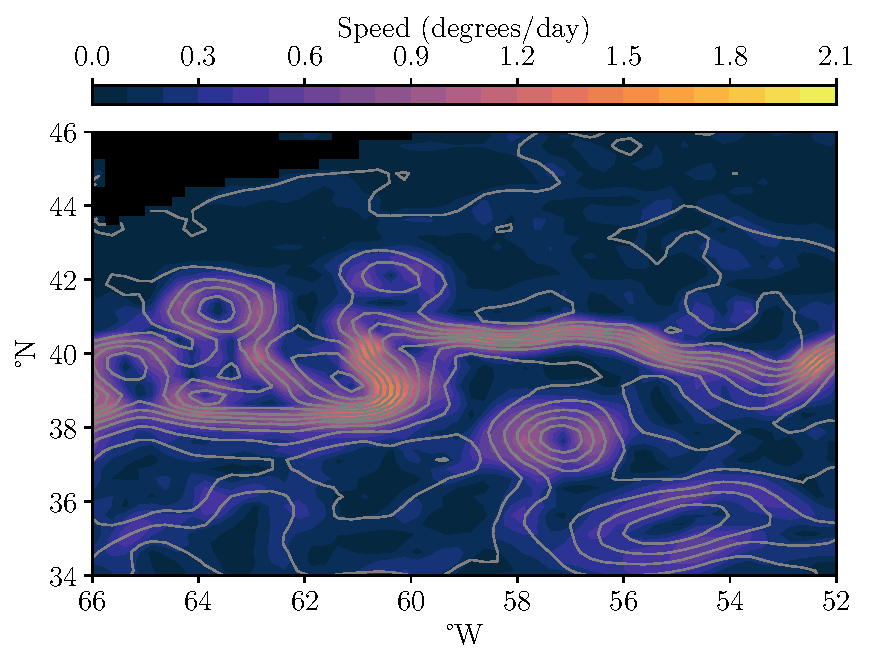
\includegraphics[width=\textwidth]{chp06_applications/figures/gulf_stream/streamlines_0}
			\caption{\(t = 0\) (midnight \DTMdisplaydate{2020}{01}{01}{})}
		\end{subfigure}
		\begin{subfigure}{0.49\textwidth}
			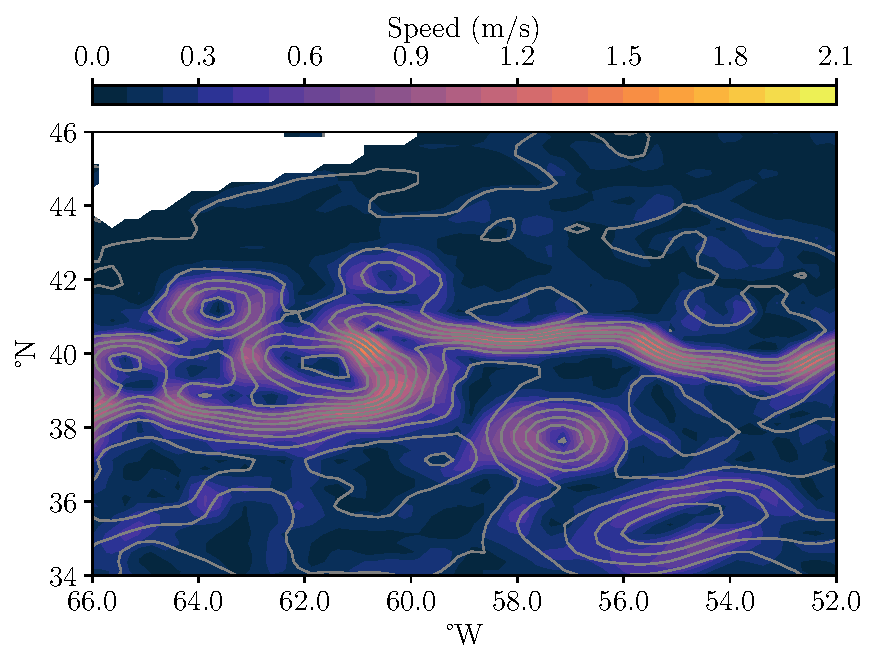
\includegraphics[width=\textwidth]{chp06_applications/figures/gulf_stream/streamlines_2}
			\caption{\(t = 2.8\) (midnight \DTMdisplaydate{2020}{01}{03}{})}
		\end{subfigure}
		\begin{subfigure}{0.49\textwidth}
			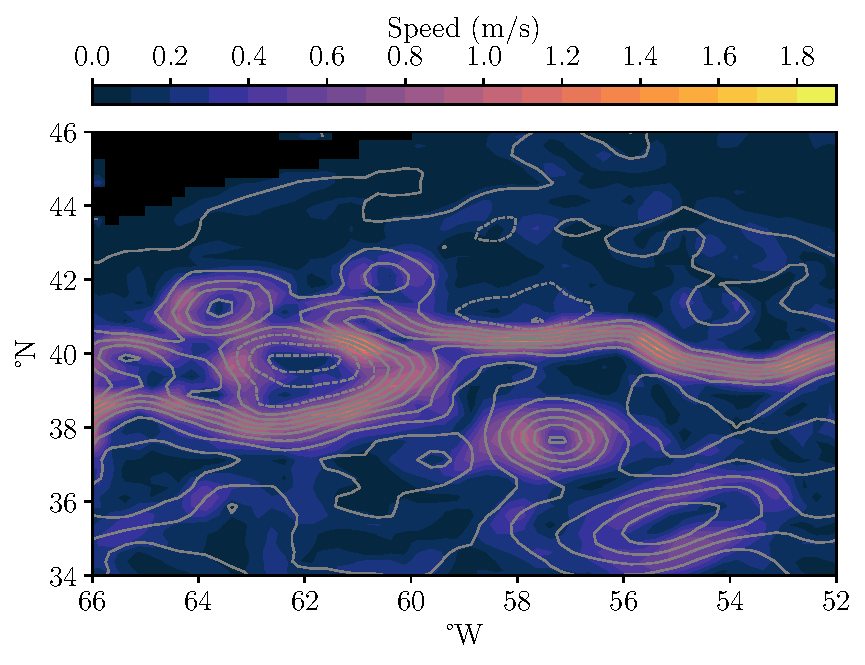
\includegraphics[width=\textwidth]{chp06_applications/figures/gulf_stream/streamlines_4}
			\caption{\(t = 4.2\) (midnight \DTMdisplaydate{2020}{01}{04}{})}
		\end{subfigure}
		\begin{subfigure}{0.49\textwidth}
			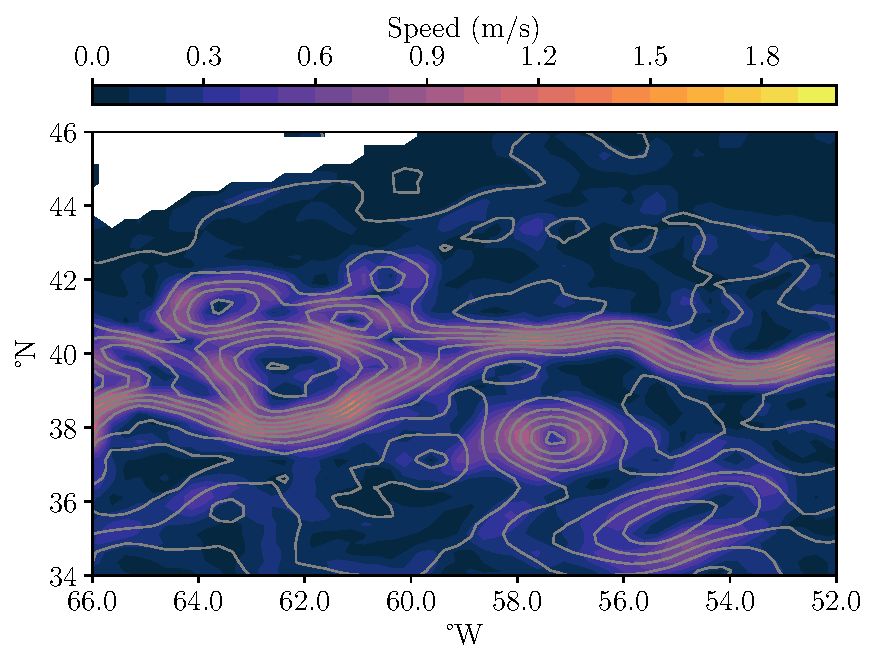
\includegraphics[width=\textwidth]{chp06_applications/figures/gulf_stream/streamlines_6}
			\caption{\(t =5.6\) (midnight \DTMdisplaydate{2020}{01}{05}{})}
		\end{subfigure}
		\caption{The absolute surface current speed (coloured) and contours of the sea-surface height (streamlines of the flow, in grey) of the Gulf Stream dataset, at various times chosen to demonstrate the formation and separation of an eddy from the stream.
			The white region indicates missing data, due to the presence of land.
			All times are in Greenwich Mean Time.}
		\label{fig:na_motive_flow}
	\end{center}
\end{figure}




The velocity data is Eulerian and unsteady (varying with time), so to predict the position of a drifter we must solve for a Lagrangian trajectory.
This requires interpolating the velocity data, for which we use a linear interpolate.
Let \(x_t \equiv \left(x_t^{(\mathrm{lon})}, x_t^{(\mathrm{lat})}\right)^{\T}\) denote the longitudinal and latitudinal position of the drifter \(t\) days after midnight \DTMdisplaydate{2020}{01}{01}.
The deterministic model for \(x_t\), constructed purely from the interpolated velocity data, is
\begin{equation}\label{eqn:natl_ode}
	\dod{}{t}\begin{bmatrix}
		x_t^{(\text{lon})} \\ x_t^{(\text{lat})}
	\end{bmatrix} = \begin{bmatrix}
		u\!\left(x^{(\mathrm{lon})}_t, x^{(\mathrm{lat})}_t, t\right) \\ v\!\left(x^{(\mathrm{lon})}_t, x^{(\mathrm{lat})}_t, t\right)
	\end{bmatrix},
\end{equation}
where \(u\) and \(v\) are the interpolated zonal and meridional velocities respectively.
In this context, we may think of \cref{eqn:natl_ode} as our ``best available'' deterministic model for the time-evolution of the drifter position; if the data (and the subsequent interpolation) were exactly correct, then \cref{eqn:natl_ode} would provide accurate predictions.
However, this is certainly not the case and there are many sources of uncertainty not accounted for by using \cref{eqn:natl_ode} alone.

The dataset additionally includes estimates for the mapping error (an estimate of variance) in the zonal and meridional velocity measurements, and in particular provides an indication of measurement error; typically the error is smaller in regions directly under satellite tracks.
To account for measurement error, we use the following stochastic model
\begin{equation}
	\dif \begin{bmatrix}
		x^{(\mathrm{lon})}_t \\ x^{(\mathrm{lat})}_t
	\end{bmatrix} = \begin{multlined}[t]
		\begin{bmatrix} u\left(x^{(\mathrm{lon})}_t, x^{(\mathrm{lat})}_t, t\right) \\ v\left(x^{(\mathrm{lon})}_t, x^{(\mathrm{lat})}_t, t\right) \end{bmatrix}\dif t \\
		+ L_r\begin{bmatrix}
			\sqrt{u_{\mathrm{err}}\left(x^{(\mathrm{lon})}_t, x^{(\mathrm{lat})}_t, t\right)} & 0                                                                                 \\
			0                                                                                 & \sqrt{v_{\mathrm{err}}\left(x^{(\mathrm{lon})}_t, x^{(\mathrm{lat})}_t, t\right)}
		\end{bmatrix} \dif W_t,
	\end{multlined}
	\label{eqn:natl_sde}
\end{equation}
where \(u_{\mathrm{err}}\) and \(v_{\mathrm{err}}\) are the interpolated error estimates for the zonal and meridional velocities (converted to \unit{\degree\per\square\day} using the same transformation as was done on the velocity data)\td{I may have messed this conversion up slightly - the error is a variance measure, so the units should be squared.}, and \(L_r = 0.25 \mathrm{\,degrees}\) is the spatial resolution of the data.



% The derivatives \(\nabla u\) of the deterministic velocity field in \cref{eqn:natl_sde} are approximated via the centred finite-differences,
% \begin{align*}
% 	\dpd{u\left({x^{(\text{lon})}}, {x^{(\text{lat})}}, t\right)}{{x^{(\text{lon})}}} & \approx \frac{u\left(x^{(\text{lon})} + L_r, x^{(\text{lat})}, t\right) - u\left(x^{(\text{lon})} - L_r, x^{(\text{lat})}, t\right)}{2 L_r},
% \end{align*}
% and similar for the remaining derivatives.



% We will now introduce an example of a differential equation model constructed from observed data, which we will use throughout this chaper, and explore further in \Cref{ch:appls}.
% In particular, the technical details of this example will be provided in \Cref{sec:appl_ocean}.

% Suppose we are interested in tracking the position of a drifter on the surface of the Gulf Stream.
% The only information we have available are measurements of the eastwards (zonal) and northwards (meridional) velocities at the surface, derived from altimetry (sea surface height) data.
% Such data is available from the European Commission`s Copernicus Marine Environment Monitoring Service.

% For the purposes of this example, assume that the position of the drifter at the initial time is known exactly\footnote{In practice, of course, this will not be the case, but this will introduce even more uncertainty into our model, furthering reinforcing the purpose of this example.}.
% Assuming that the interpolated data provided an accurate model of the sea surface velocity, the position \(x_t\) of the drifter on the surface at time \(t\) is the solution to the ordinary differential equation
% \begin{equation}\label{eqn:na_motiv_ode}
% 	\dod{x_t}{t} = u\left(x_t, t\right),
% \end{equation}
% subject to the known initial position \(x_0\), where \(u\) is the appropriately interpolated surface velocity data.
% To illustrate the time-varying dynamics of the Stream, \Cref{fig:na_motiv_flow} plots contours the sea-surface height, which correspond to the time-varying streamfunction of the flow, and therefore solutions to \cref{eqn:na_motiv_ode}, at various times.
% An important feature of the flow is that there are significantly different qualitative regimes; there is the rapidly moving stream itself, the eddies that are shed and slow moving, and isotropic regions in between where the current is comparatively slow.



% We can easily solve \cref{eqn:na_motiv_ode} numerically to obtain a predicted position for our drifter on day \(t\).
% % We term \cref{eqn:na_motiv_ode} the \emph{deterministic model}, since given the data we have available, it serves as our best purely deterministic model for the position of the drifter.
% Suppose that our drifter begins within the stream itself, at \(x_0 = \left(-60.5, 39\right)^{\T}\), \Cref{fig:na_motiv_det} plots the resulting trajectory (in white) obtained by solving \cref{eqn:na_motiv_ode} numerically, over the span of 7 days starting from midnight \DTMdisplaydate{2020}{01}{01}{}.
% Based on this model, we expect that the drifter will follow the Stream, which can inform efforts to locate the drifter.

% \begin{figure}
% 	\begin{center}
% 		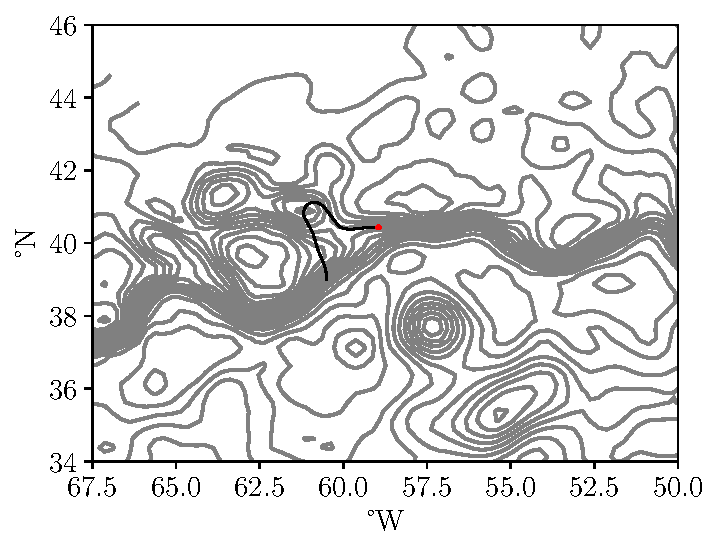
\includegraphics[width=\textwidth]{chp06_applications/figures/gulf_stream_motivation/det_traj.pdf}
% 		\caption{The time evolution of the solution (obtained by numerically integrating the velocity data) to the deterministic system corresponding to \cref{eqn:natl_sde}, from initial condition \(x_0 = \left(-60.5, 39\right)^{\T}\) from 01/01/2021 (\(t = 0\)) to 08/01/2021 (\(t = 8\)).
% 			Contours of the sea surface height at the final time \(t = 8\) are included in grey to indicate the position of the Gulf Stream and nearby eddies in the flow.}
% 		\label{fig:na_motiv_det}
% 	\end{center}
% \end{figure}

% To improve our predictions of the future position of the drifter, we should attempt to account for this uncertainty in our model \cref{eqn:na_motiv_ode}.
% The altimetry-derived data also includes measures of error in each component of the velocity at each spatiotemporal gridpoint, so we can use these measurements to model the ongoing observational error in \(u\).
% We can extend \cref{eqn:na_motiv_ode} as a stochastic differential equation, where the unresolved uncertainty is parameterised as a white-noise process scaled by measurement error.
% Specifically, we formulate the drifter position as \cref{eqn:natl_sde} in \Cref{sec:gulf_stream}, which is explained in more detail in that section.
% For our purposes here, \cref{eqn:natl_sde} is a stochastic differential equation analogy of \cref{eqn:natl_sde} that we can solve numerically to obtain approximate solution samples.

% \Cref{fig:na_motiv_rels} shows us the result of numerically solving a stochastic differential equation formulation (specifically ) of the Lagrangian trajectory model.
% This is a ``more correct'' model than the deterministic counterpart, in the sense that it is attempting to account for the unknowable measurement error and unresolved subgrid effects.
% Each realisation here could correspond to our drifter, and we see a far different picture than the deterministic model alone provided.
% Qualitatively, rather than following the Stream itself, a proportion of particles are caught in one of two eddies which have formed and broken off from the Stream.

% \begin{figure}
% 	\begin{center}
% 		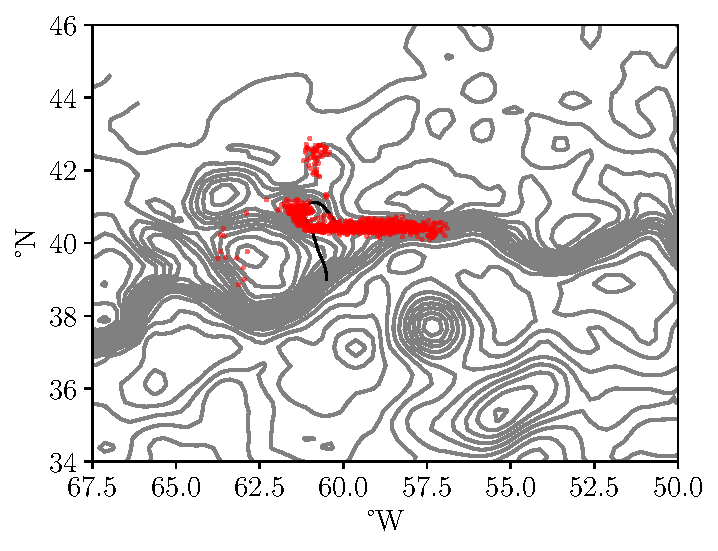
\includegraphics[width=\textwidth]{chp06_applications/figures/gulf_stream_motivation/num_rels.pdf}
% 		\caption{The same visualisation of the deterministic behaviour of the Gulf Stream example as \Cref{fig:na_motive_det}, but with the final positions of 10000 numerical realisations of a stochastic model, each indicated by a red point.}
% 		\label{fig:na_motiv_rels}
% 	\end{center}
% \end{figure}

% Although deterministic models are often easier to work with analytically and far more efficient to solve numerically, these models are limited.
% By explicitly accounting for uncertainty with a stochastic, we can expand the scope of our model and provide more realistic and useful predictions, at the cost of a more complicated model.
% This idea of introducing stochastic components into a deterministic model to account for unresolved and unknown aspects has been used extensively in recent times across scientific applications, notably atmospheric, climate, and oceanographic modelling.
% We provide an overview of this so-called stochastic parameterisation in the next section, and highlight how the work of this thesis fits in with the needs of that field.



\subsection{Exploring a single trajectory}
In this example, we shall consider a fixed initial condition.
Suppose that at midnight \DTMdisplaydate{2021}{01}{01}, the drifter is located within the stream  at longitude \(60.5^\circ\) west and \(39^\circ\) north.
We accordingly consider the evolution of the models \cref{eqn:natl_ode} and \cref{eqn:natl_sde} with the initial condition \(x_0 = (-60.5, 39)^{\T}\).

\begin{figure}
	\begin{center}
		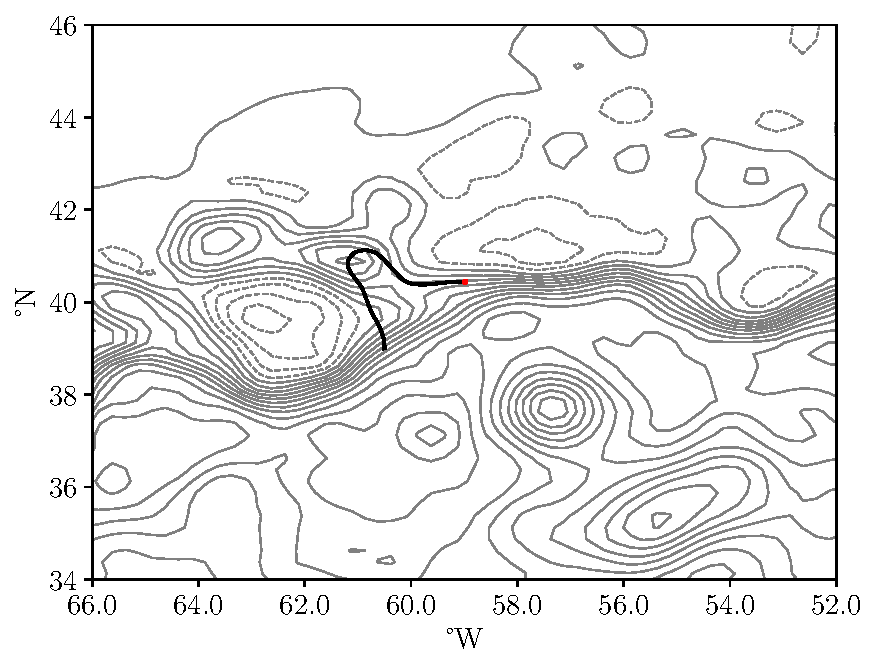
\includegraphics[width=\textwidth]{chp06_applications/figures/gulf_stream/det_traj.pdf}
		\caption{The solution to \cref{eqn:natl_ode} with initial condition \((-60.5, 39)^{\T}\) from midnight \DTMdisplaydate{2021}{01}{01} to midnight \DTMdisplaydate{2021}{01}{08}, corresponding to a drifter on the surface of the Gulf Stream.
			Contours of the sea surface height at the final time are included in grey, which correspond to contours of the streamfunction at that time.}
		\label{fig:natl_det_traj}
	\end{center}
\end{figure}

By solving the deterministic model \cref{eqn:natl_ode} numerically, we predict the position of the drifter after \(t = 7\) days (at midnight \DTMdisplaydate{2021}{01}{08}) and show the time-evolution of the solution trajectory in \Cref{fig:natl_det_traj}.
The drifter is transported by the stream.






% \begin{figure}
% 	\begin{center}
% 		\begin{subfigure}{\textwidth}
% 		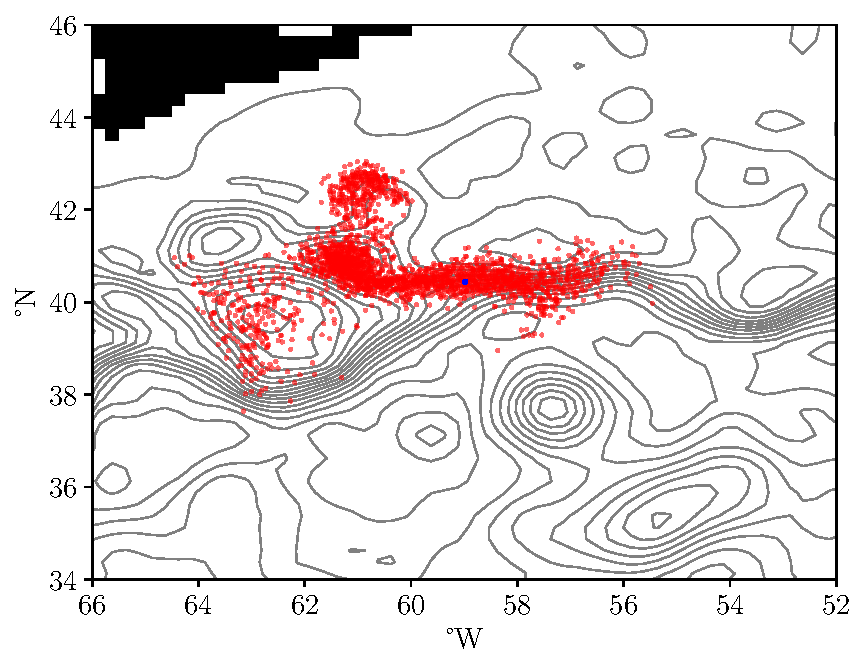
\includegraphics[width=\textwidth]{chp06_applications/figures/gulf_stream/traj_stoch_rels.pdf}
% 			\caption{The final position of \(N = 10000\) samples of the stochastic solution.}
% 		\end{subfigure}

% 	\begin{subfigure}{\textwidth}
% 		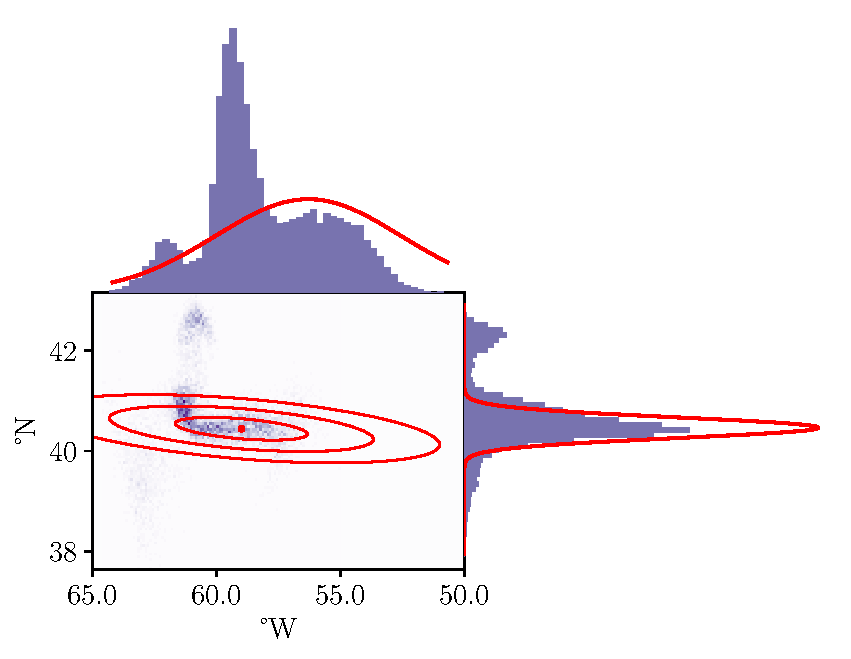
\includegraphics[width=\textwidth]{chp06_applications/figures/gulf_stream/traj_stoch_joint_gauss.pdf}
% 		\caption{}
% 		\end{subfigure}

% 		\caption{Samples of the solution to the stochastic model \cref{eqn:natl_sde} with initial condition \((-60.5, 39)^{\T}\) from DATE to DATE, corresponding to a drifter on the surface of the Gulf Stream.
% 		Contours of the sea surface height at the final time are included in grey, which correspond to contours of the streamfunction at that time.}
% 		\label{fig:natl_stoch_rels}
% 	\end{center}
% \end{figure}





\begin{figure}
	\begin{center}
		\begin{subfigure}{\textwidth}
			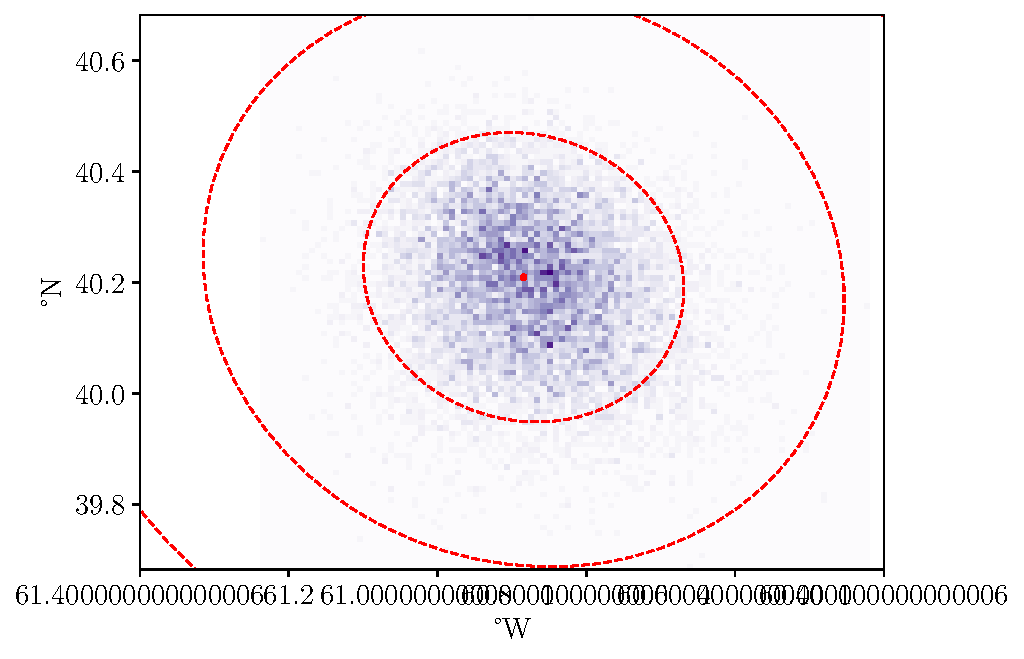
\includegraphics[width=0.49\textwidth]{chp06_applications/figures/gulf_stream/traj_stoch_em_1.pdf}
			\caption{\(t = 1\) (midnight \DTMdisplaydate{2021}{02}{01}))}
		\end{subfigure}

		\begin{subfigure}{\textwidth}
			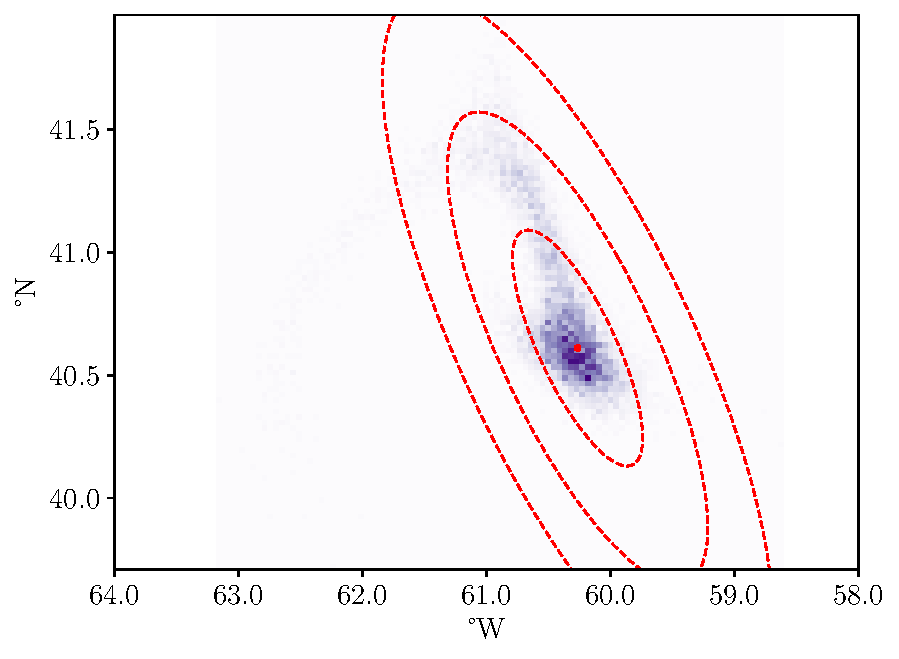
\includegraphics[width=0.49\textwidth]{chp06_applications/figures/gulf_stream/traj_stoch_em_4.pdf}
			\caption{\(t = 4\) (midnight \DTMdisplaydate{2021}{05}{01}))}
		\end{subfigure}

		\begin{subfigure}{\textwidth}
			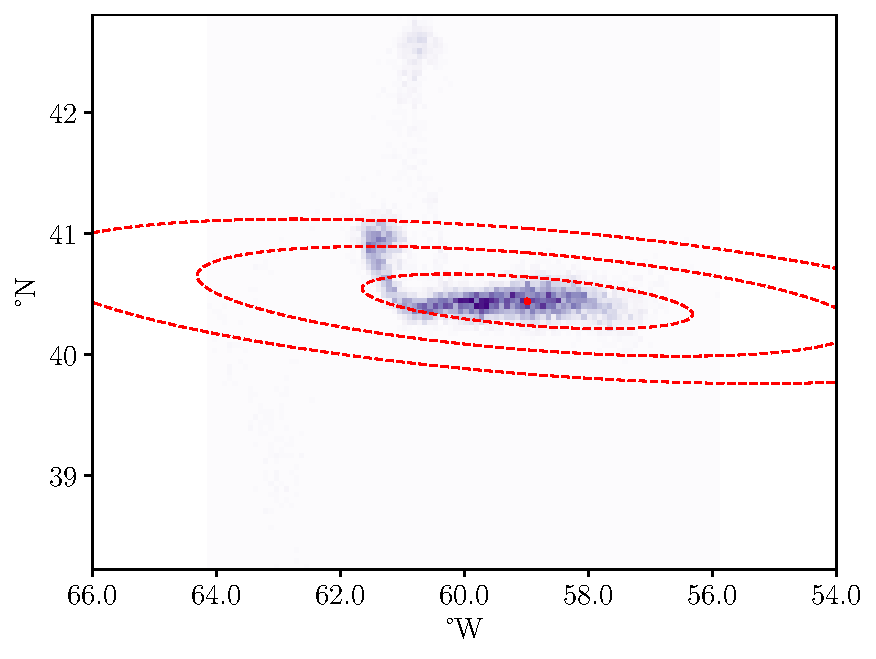
\includegraphics[width=0.49\textwidth]{chp06_applications/figures/gulf_stream/traj_stoch_em_7.pdf}
			\caption{\(t = 7\) (midnight \DTMdisplaydate{2021}{08}{01}))}
		\end{subfigure}
		% \includegraphics[width=\textwidth]{}
		\caption{}
		\label{fig:}
	\end{center}
\end{figure}



% \begin{table}
% 	\begin{tabular}{|c|c|c|c|c|}
% 		\hline
% 		\multirow{2}{*}{Time}      & \multirow{2}{*}{Algorithm pair} & \multicolumn{3}{c|}{Metric}                                           \\ \cline{3-5}
% 		                           &                                 & Strong error                & Hellinger distance & Wasserstein metric \\ \hline
% 		\multirow{3}{*}{\(t = 1\)} & Gaussian \& EM                  &                             &                    &                    \\ \cline{2-5}
% 		                           & Gaussian \& FP                  &                             &                    &                    \\ \cline{2-5}
% 		                           & EM \& FP                        &                             &                    &                    \\ \hline
% 	\end{tabular}
% 	\caption{Performance metrics for the Gaussian approximation against Euler-Maruyama samples and a number solution of the Fokker-Planck equation, for the Gulf Stream trajectory.}
% 	\label{tab:natl_gauss_perform}
% \end{table}



\begin{figure}
	\begin{center}
		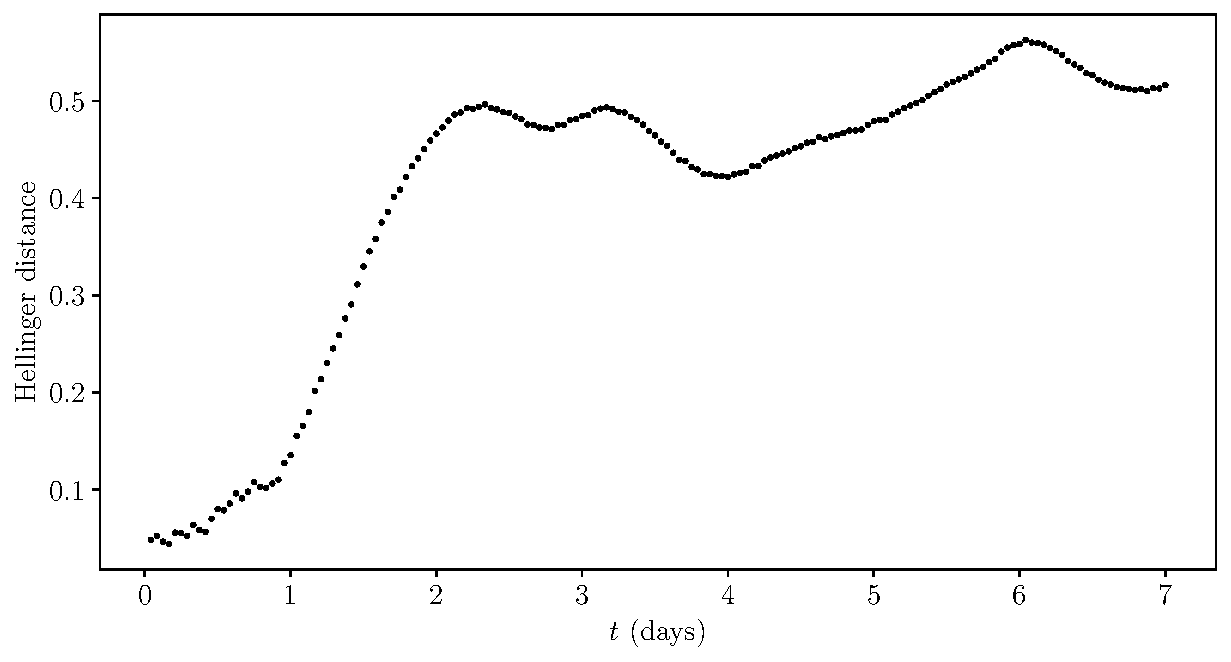
\includegraphics[width=\textwidth]{chp06_applications/figures/gulf_stream/traj_stoch_hell_dist.pdf}
		\caption{The Hellinger distance between \(N = 10000\) Euler-Maruyama samples of \cref{eqn:natl_sde} and the Gaussian process solution to the linearisation, \(t\) days after midnight \DTMdisplaydate{2021}{01}{01}.}
		\label{fig:}
	\end{center}
\end{figure}





\subsection{Stochastic sensitivity}


\Cref{fig:na_s2} plots the stochastic sensitivity field





\begin{figure}
	\begin{center}
		\begin{subfigure}[t]{0.49\textwidth}
			\includegraphics[width=\textwidth]{chp06_applications/figures/gulf_stream/S2_field_grid}
			\caption{The stochastic sensitivity \(S^2\).}
		\end{subfigure}
		\begin{subfigure}[t]{0.49\textwidth}
			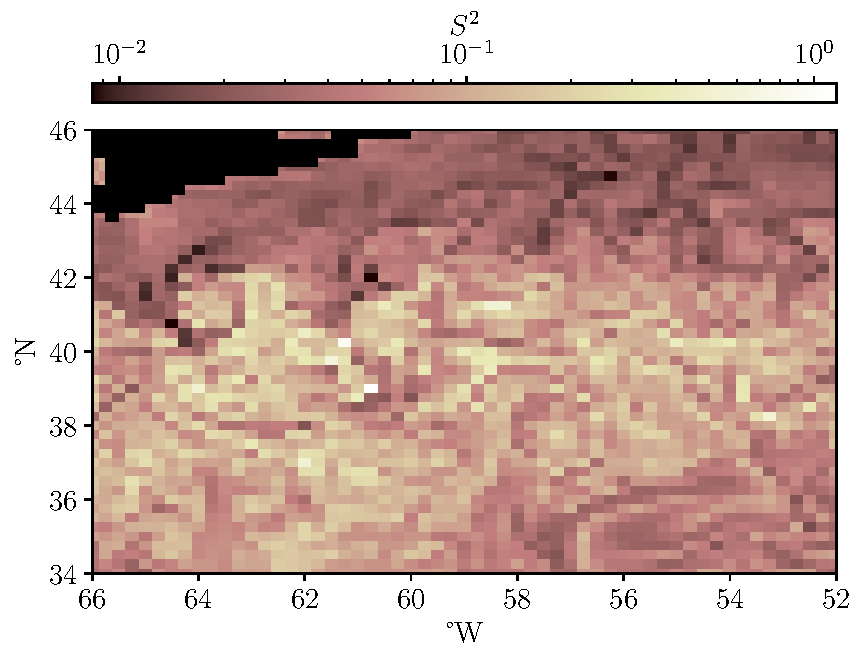
\includegraphics[width=\textwidth]{chp06_applications/figures/gulf_stream/s2min_field_grid}
			\caption{The minimum eigenvalue of the covariance matrix.}
		\end{subfigure}
		\begin{subfigure}[t]{0.49\textwidth}
			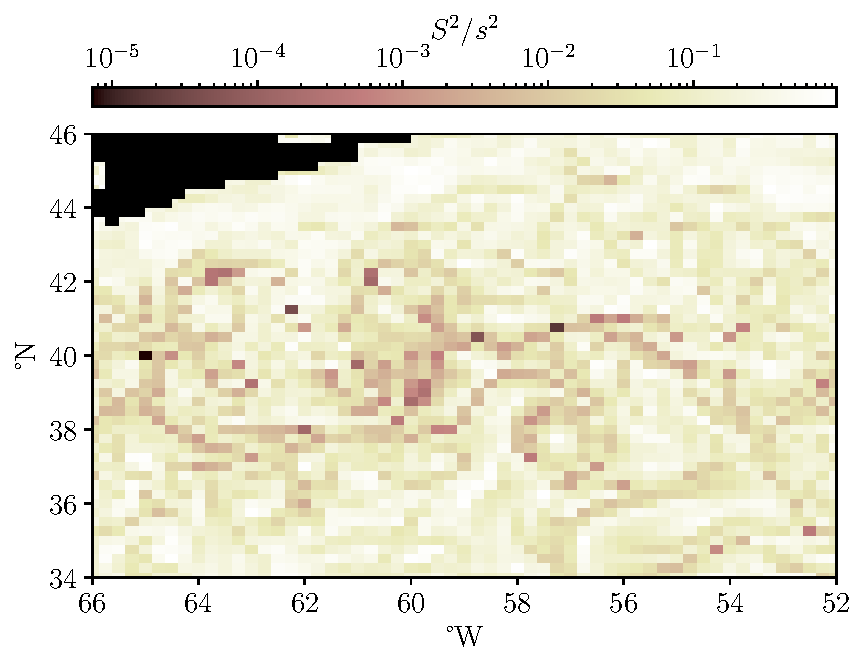
\includegraphics[width=\textwidth]{chp06_applications/figures/gulf_stream/ratio_field_grid}
			\caption{The ratio of the stochastic sensitivity value (maximum eigenvalue) and the minimum eigenvalue of the covariance matrix, which captures the `narrowness' of the linearised distribution.}
		\end{subfigure}
		\begin{subfigure}[t]{0.49\textwidth}
			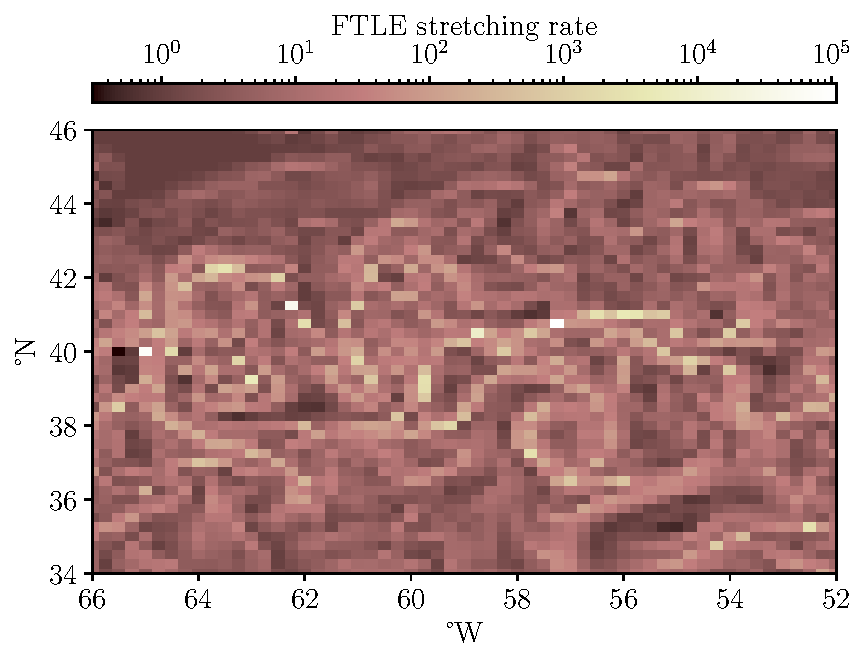
\includegraphics[width=\textwidth]{chp06_applications/figures/gulf_stream/ftle_field_grid}
			\caption{The stretching rate field used in the FTLE calculation.}
		\end{subfigure}
		% \begin{subfigure}[t]{0.49\textwidth}
		% 	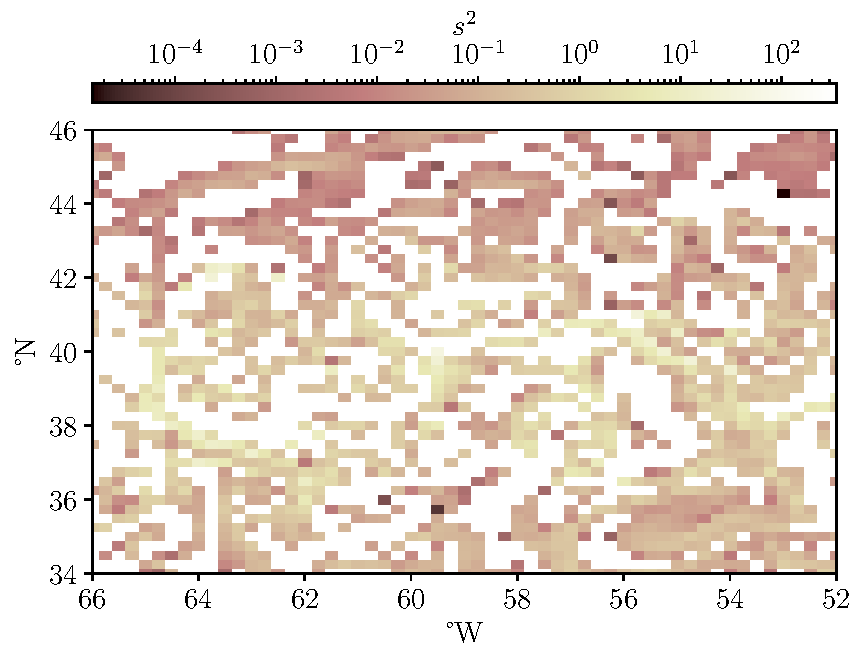
\includegraphics[width=\textwidth]{chp06_applications/figures/gulf_stream/cov_field_grid}
		% 	\caption{The \((1,2)\)th entry of the covariance matrix, corresponding to the covariance between coordinates.
		% 		White indicates regions in which the entry is zero.}
		% \end{subfigure}
		\caption{Fields computed from the linearisation covariance matrix on a grid of initial conditions (at the \(0.25^\circ \times 0.25^\circ\) resolution of the velocity data).
			Note that values near the boundaries of the data and the land are not trustworthy, as the Gaussian approximations do not account for these boundaries.}
		\label{fig:na_s2}
	\end{center}
\end{figure}




\begin{figure}
	\begin{center}
		\begin{subfigure}[t]{\textwidth}
			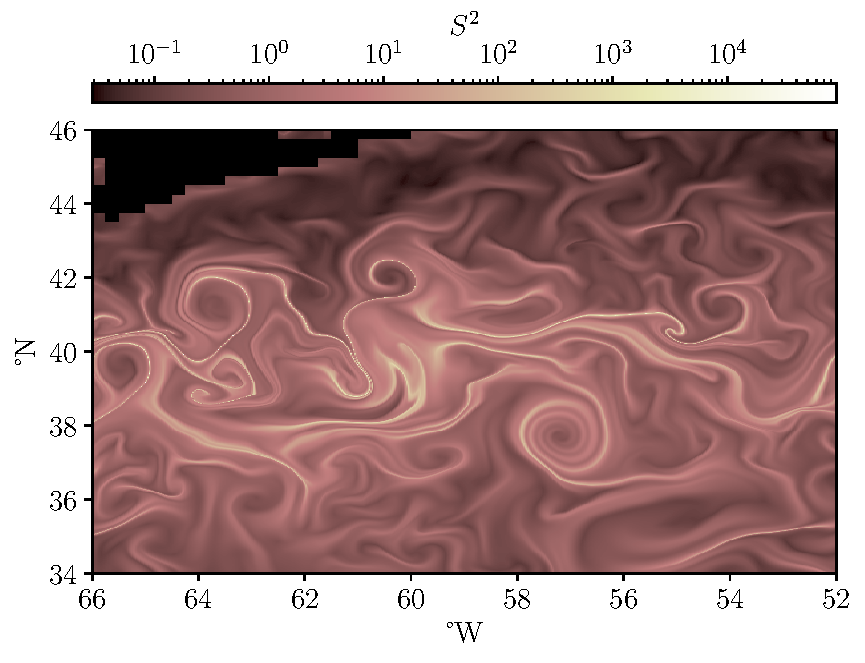
\includegraphics[width=\textwidth]{chp06_applications/figures/gulf_stream/S2_field_high}
			\caption{The stochastic sensitivity \(S^2\).}
		\end{subfigure}
		\begin{subfigure}[t]{0.49\textwidth}
			\includegraphics[width=\textwidth]{chp06_applications/figures/gulf_stream/s2_field_high}
			\caption{The minimum eigenvalue of the covariance matrix.}
		\end{subfigure}
		\begin{subfigure}[t]{0.49\textwidth}
			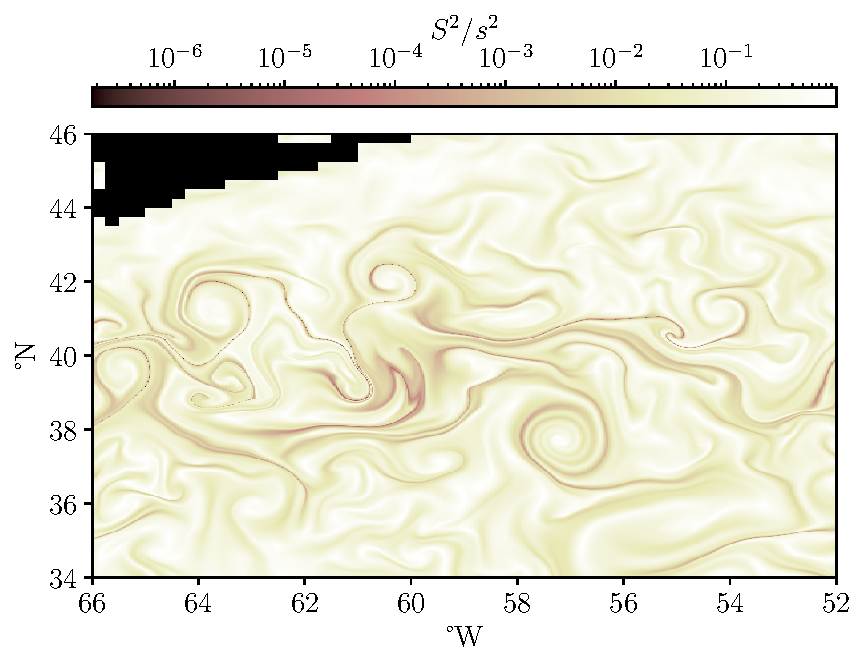
\includegraphics[width=\textwidth]{chp06_applications/figures/gulf_stream/ratio_field_high}
			\caption{The ratio of the stochastic sensitivity value (maximum eigenvalue) and the minimum eigenvalue of the covariance matrix, which captures the `narrowness' of the linearised distribution.}
		\end{subfigure}
		% \begin{subfigure}[t]{0.49\textwidth}
		% 	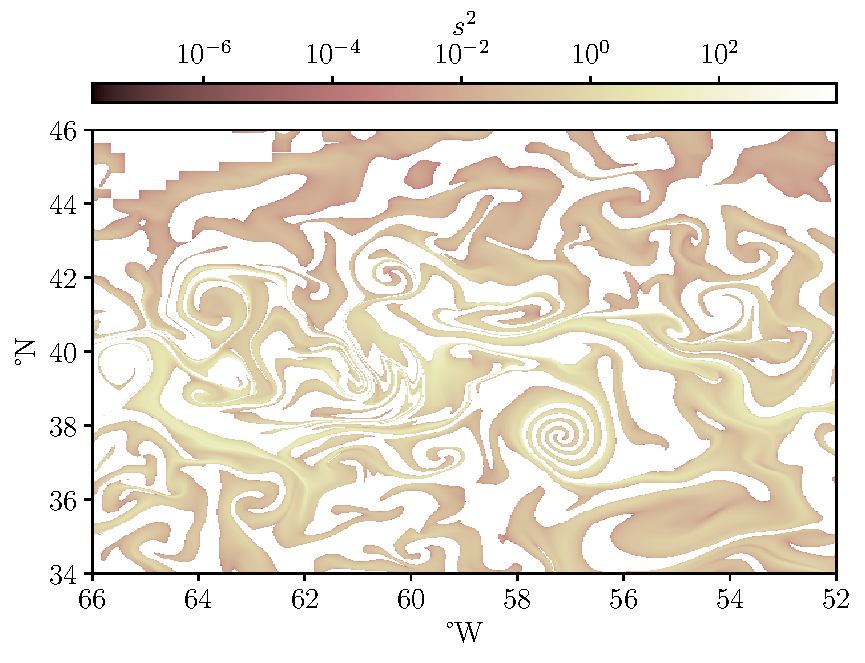
\includegraphics[width=\textwidth]{chp06_applications/figures/gulf_stream/cov_field_high}
		% 	\caption{The \((1,2)\)th entry of the covariance matrix, corresponding to the covariance between coordinates.
		% 		White indicates regions in which the entry is zero.}
		% \end{subfigure}
		\caption{Fields computed from the linearisation covariance matrix on a grid of initial conditions, in the same arrangement as \Cref{fig:na_s2} but at a higher resolution of \(0.025^\circ \times 0.025^\circ\).
			Note that values near the boundaries of the data and the land are not trustworthy, as the Gaussian approximations do not account for these boundaries.}
		\label{fig:na_s2_high}
	\end{center}
\end{figure}


\subsection{The mixture model}




\section{Empirical model of sea-surface winds}
\td{Possibly something funky to try - use the observed data to construct the FLOW MAP, and then compute based purely on that!! The paper by \cite{Sura_2003_StochasticAnalysisSouthern} basically interpolates the data then uses finite differences and statistical averaging to find the ODE. But we can avoid that step entirely by just treating the data!}

Empirical, or data-driven, stochastic models are used heavily in climate science, where components of the model are derived by fitting to time series of observed data.
In this section, we follow the method of \citet{EggerJonsson_2002_DynamicModelsIcelandic} and \citet{Sura_2003_StochasticAnalysisSouthern} to construct from observed data a stochastic differential equation model for the time evolution of sea surface wind velocities.

Consider an \(n\)-dimensional state variable \(x_t\) governed by the It\^o SDE
\begin{equation}\label{eqn:sde_emp}
	\dif x_t = A(x_t) + B(x_t)\dif W_t,
\end{equation}
where \(W_t\) is an \(n\)-dimensional Wiener process and the coefficients \(A \colon \R^n \to \R^n\) and \(B \colon \R^n \to \R^{n\times n}\) are permitted to vary with state but not time.
To determine the drift and diffusion directly from observed data, we consider the statistical definitions of the coefficients:
\begin{subequations}\label{eqn:sde_coef_stat}
	\begin{align}
		A(x)          & = \lim_{\delta t \to 0}\frac{1}{\delta t}\avg{x_{t + \delta t} - x} \label{eqn:sde_coef_stat_drift}                                                \\
		B(x)B(x)^{\T} & = \lim_{\delta t \to 0}\frac{1}{\delta t}\avg{\left(x_{t + \delta} - x\right)\left(x_{t + \delta} - x\right)^{\T}}, \label{eqn:sde_coef_stat_diff}
	\end{align}
\end{subequations}
where the expected values are taken over all trajectories solving \cref{eqn:sde_emp} with \(x_{t} = x\).
The expressions in \cref{eqn:sde_coef_stat} arise by considering the Fokker-Planck equation corresponding to \eqref{eqn:sde_emp} \citehere.

Now suppose that we have a collection of \(K\) time series, each corresponding to a solution trajectory of \cref{eqn:sde_emp} and evaluated at (possibly non-uniform) times \(t_0, t_1, \dotsc, t_n\).
Let the \(k\)th time series be denoted by
\[
	\set{X_{0}^{(k)}, X_{1}^{(k)}, \dotsc, X_{n}^{(k)}}.
\]
The definitions in \cref{eqn:sde_coef_stat} are only correct in the limit as \(\delta t\) approaches zero, which we cannot obtain from our discrete-time data, and involves expectations of the theoretical solution to \eqref{eqn:sde_emp}.
However, we can approximate the expressions using a finite difference for the limit and binned sample estimates for the expectations.




\section{Epidemiology}


\subsection{A very brief overview of population processes}


A common model for population process are continuous-time Markov chains (CTMCs)

\begin{enumerate}
	\item Initialise \(X = X_0\), the initial state of the process.
	      If the initial state is uncertain, sample \(X\) from the initial state distribution.

	\item Sample the time \(\tau\) to the next event as
	      \[
		      \tau \isExp{\sum_{\substack{l \in \R^n \\ l \neq 0,\, y + l \in \mathcal{S}}}{q\!\left(X, X + l\right)}},
	      \]
	      and set \(t = t + \tau\).

	\item If \(t > T\), terminate.
	      Otherwise, sample the next state from the set of possible transitions \(\setc{l \in \R^n}{l \neq 0,\, y + l \in \mathcal{S}}\), where the probability of transitioning from \(X\) to \(X + l\) is given by
	      \[
		      \frac{q\!\left(X, X + l\right)}{\sum_{\substack{k \in \R^n \\ k \neq 0,\, y + k \in \mathcal{S}}}{q\!\left(X, X + k\right)}}.
	      \]
	      Set \(X\) to this state.

	\item Repeat Steps 2 and 3 until the sample path is terminated.

\end{enumerate}
The result is a single sample \(X\) of the population process at time \(T\).
The sum is taken across all the possible transitions from the current state.
Note that typically most of these rates are zero, so the sum does not need to be taken over the entire state space.

\subsection{Large population diffusion limits}

A population process is \emph{density dependent} (in the sense of \citet{Kurtz_1970_SolutionsOrdinaryDifferential}) if there is a parameter \(N\) such that
\begin{equation}
	q\!\left(n, n+l\right) = Nf\!\left(\frac{n}{N}, l\right),
	\label{eqn:ctmc_dens_dep}
\end{equation}
where \(f\) is a suitable function and \(n, n+l \in \mathcal{S}\).
Typically, \(N\) is related to the size of the system and \(n / N\) is a population density.
The condition in \cref{eqn:ctmc_dens_dep} states that the transition rates of the process \(X_t\) depends on \(X_t\) itself only through the density \(X_t / N\).

Let \(Y_t^{(N)}\) describe the \(n\)-dimensional density process, i.e. with \(i\)th element \(X_t^{(i)} / N\).
Theorem 3.1 of \citet{Kurtz_1970_SolutionsOrdinaryDifferential} establishes that in the large population limit \(N \to \infty\), the density process \(Y_t^{(N)}\) converges in probability to a deterministic trajectory \(Y_t^{(\infty)}\) solving the ODE
\begin{equation}
	\dod{Y_t^{(\infty)}}{t} = Q\!\left(Y_t^{(\infty)}\right), \quad Y_0^{(\infty)} = X_0 / N,
	\label{eqn:ctmc_dens_dep_ode}
\end{equation}
where
\[
	Q\!\left(y\right) = \sum_{\substack{l \in \R^n \\ l \neq 0,\, y + l \in \mathcal{S}}}{l f\!\left(y, l\right)}.
\]
For large \(N\), the density process has small variation and is ``close'' to the deterministic solution to \cref{eqn:ctmc_dens_dep_ode}.
This result is analogous to that for small noise SDEs; the solution to a stochastic differential equation formally converges to that of a deterministic system (involving only the drift term) in the limit of small noise, which is a result established by large deviations principles \citep[e.g]{FreidlinWentzell_1998_RandomPerturbationsDynamical}.

\citet{Kurtz_1971_LimitTheoremsSequences} then established a stronger result, showing that the variation of the density process about this deterministic limit is captured by an It\^o diffusion.
Define the scaled process
\[
	Z_t^{(N)} = \sqrt{N}\left(Y_t^{(N)} - Y_{t}^{(\infty)}\right),
\]
then Theorem 3.5 of \citet{Kurtz_1971_LimitTheoremsSequences} proves that \(Z_t^{(N)}\) converges in distribution (weakly) to an It\^o diffusion \(Z_t^{(\infty)}\) solving
\begin{equation}
	\dif Z_t^{(\infty)} = \nabla Q\!\left(Y_t^{(\infty)}\right) Z_t^{(\infty)}\dif t + G\!\left(Y_t^{(\infty)}\right)\dif W_t, \quad Z_0^{(\infty)} = 0,
	\label{eqn:ctmc_dens_dep_sde}
\end{equation}
where \(W_t\) is an \(n\)-dimensional Wiener process and the \(n \times n\) diffusion matrix \(G\) is such that
\begin{equation}
	\left[G\!\left(y\right)G\!\left(y\right)^{\T}\right]_{ij} = \sum_{\substack{l \in \R^n \\ l \neq 0,\, y + l \in \mathcal{S}}}{l_i l_j f\!\left(y,l\right)}
	\label{eqn:ctmc_dens_dep_sde_diff_cond}
\end{equation}
Any choice of diffusion matrix \(G\) such that \cref{eqn:ctmc_dens_dep_sde_diff_cond} is satisfied will result in a statistically identical diffusion process \(Z_0^{(\infty)}\).

The limiting SDE \cref{eqn:ctmc_dens_dep_sde} is equivalent to the unscaled SDE
\begin{equation}
	\dif L_t^{(N)} = \left[Q\!\left(Y_t^{(\infty)}\right) + \frac{1}{\sqrt{N}} \nabla Q\!\left(Y_t^{(\infty)}\right)\left(L_t^{(N)} - Y_t^{(\infty)}\right)\right]\dif t + \frac{1}{\sqrt{N}}G\!\left(Y_t^{(\infty)}\right)\dif W_t,
	\label{eqn:ctmc_sde_lin_lim}
\end{equation}
which is a linearisation of the nonlinear SDE
\begin{equation}
	\dif \hat{Y}^{(N)}_t = Q\!\left(\hat{Y}^{(N)}_t\right)\dif t + \frac{1}{\sqrt{N}}G\!\left(\hat{Y}_t^{(N)}\right)\dif W_t
	\label{eqn:ctmc_sde_lim_nonlin}
\end{equation}
about the deterministic limit \(Y_t^{(\infty)}\).
There is intuition behind the choices of drift and diffusion in \cref{eqn:ctmc_sde_lim_nonlin}.
For sufficiently large \(N\), the drift term \(Q\) captures the average (macroscopic) behaviour of the density process.
The diffusion term captures the microscopic behaviour resulting from individual transition events, and the uncertainty in this is parameterised with the Wiener process \(W_t\).




\td{Explain how this is analogous to the proceeding work}
However, a key difference is that in the SDE linearisation procedure, we start from a continuous state-space process and arrive at a continuous state-space process in the limit.
Whereas, in the CTMC diffusion limit, the converging process is on a \emph{discrete} state-space and the limit is on a continuous one.




Thus, we expect that the mixture model algorithm we have described may find a place in moderate-population compartmental models, where the population is large enough to be ``reasonably'' approximated by the continuum and SDE equations, but small enough to exhibit non-Gaussian behaviour.
Regardless, our error bound derived in \Cref{ch:linear_theory} still has a place in this literature.



\subsection{Example 1: the SIR model}
Assume a fixed population of \(N\) individuals, each classified into one of three compartments: susceptible (\(S\)) and infected (\(I\)), and recovered/removed (\(R\)).
At any time, the number of removed individuals can be computed as \(R = N - S - I\), so we only need to specify a two-dimensional model for the number of susceptible and infected individuals.
Such a process can model the spread of a disease in a homogeneously mixing population in which susceptible individuals become infected upon contact with infected individuals, and once infected individuals recover they are no longer infectious or susceptible to reinfection.
The state space is then
\[
	\mathcal{S} = \setc{\left(s,i\right)}{s,i \in \set{0,1,\dotsc,N}, \, s + i \leq N},
\]
where the number of recovered individuals at any time is \(N - S - I\).
The events and the corresponding transition probabilities are described in \Cref{fig:sir_transition}.

\usetikzlibrary{automata,positioning,arrows}
\tikzset{->, node distance = 2cm}
\begin{figure}
	\begin{center}
		\begin{tabular}{|c|c|c|c|}
			\hline
			Transition & \multicolumn{2}{c|}{Event} & Rate \(\lambda_i\)                                                    \\ \hline
			1          & Infection                  & \(\left(S, I\right) \to \left(S-1, I + 1\right)\) & \(\beta S I / N\) \\ \hline
			2          & Recovery                   & \(\left(S,I\right) \to \left(S, I - 1\right)\)    & \(\gamma I\)      \\ \hline
		\end{tabular} \\
		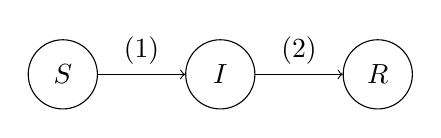
\begin{tikzpicture}
			\node[state] (S) {\(S\)};
			\node[state, right of = S] (I) {\(I\)};
			\node[state, right of = I] (R) {\(R\)};
			\draw (S) edge[above] node{(1)} (I)
			(I) edge[above] node{(2)} (R);
		\end{tikzpicture}
		\caption{Transition probabilities of the SIR compartmental model.}
		\label{fig:sir_transition}
	\end{center}
\end{figure}
The population process is density dependent, with
\[
	f\left((s,i), l\right) = \begin{cases}
		\beta s i, & \text{if } l = \left(-1, 1\right), \\
		\gamma i,  & \text{if } l = \left(0,-1\right)   \\
		0,         & \text{otherwise}.
	\end{cases}
\]
Let \(X_t^{(N)} = \left(S_t / N, I_t / N\right)\) denote the proportion of susceptible and infected individuals and at time \(t\).
The corresponding deterministic differential equation approximation is
\[
	\dod{X_t^{(\infty)}}{t} = \begin{bmatrix}
		-\beta X_t^{(\infty,1)} X_t^{(\infty, 2)} \\
		\beta X_t^{(\infty,1)} X_t^{(\infty, 2)} -\gamma X_t^{(\infty, 2)}
	\end{bmatrix},
\]
where \(X_t^{(\infty)} \equiv \left(X_t^{(\infty, 1)}, X_t^{(\infty, 2)}\right)^{\T}\).
Consider the scaling
\[
	Z_t^{(N)} = \sqrt{N}\left(X_t^{(N)} - X_t^{(\infty)}\right),
\]
then \citet{Kurtz_1971_LimitTheoremsSequences} establish that in the limit \(N \to \infty\), the scaled process \(Z_t^{(N)}\) will converge in distribution to the It\^o diffusion \(Z_t^{(\infty)}\) solving
\begin{equation}
	\dif Z_t^{(\infty)} = \begin{bmatrix}
		-\beta X_t^{(\infty, 2)} & -\beta X_t^{(\infty, 1)}         \\
		\beta X_t^{(\infty, 2)}  & \beta X_t^{(\infty, 1)} - \gamma
	\end{bmatrix} Z_t^{(\infty)}\dif t + g\!\left(X_t^{(\infty)}\right)\dif W_t
	\label{eqn:sir_diff_limit}
\end{equation}
where the diffusion matrix \(G\) satisfies
\[
	g\!\left(X_t^{(\infty)}\right)g\!\left(X_t^{(\infty)}\right)^{\T} = \begin{bmatrix}
		\beta X_t^{(\infty, 1)} X_t^{(\infty, 2)}  & -\beta X_t^{(\infty, 1)} X_t^{(\infty, 2)}                              \\
		-\beta X_t^{(\infty, 1)} X_t^{(\infty, 2)} & \beta X_t^{(\infty, 1)} X_t^{(\infty, 2)} + \gamma X_{t}^{(\infty, 2)}.
	\end{bmatrix}
\]
Any choice of \(g\) satisfying this property will result in a statistically identical diffusion process, so we take
\[
	g\!\left(X_t^{(\infty)}\right) = \begin{bmatrix}
		\sqrt{\beta X_t^{(\infty, 1)} X_t^{(\infty, 2)}}  & 0                               \\
		-\sqrt{\beta X_t^{(\infty, 1)} X_t^{(\infty, 2)}} & \sqrt{\gamma X_t^{(\infty, 2)}}
	\end{bmatrix}.
\]
The stochastic differential equation \cref{eqn:sir_diff_limit} is a linear in the same form as the linearisation \cref{eqn:linear_sde} considered in \Cref{ch:linear_theory}, and so is solved by the Gaussian process
\[
	Z_t^{(\infty)} \isGauss{0,\, \Sigma_0^t\!\left(X_0^{(\infty)}\right)},
\]
where \(\Sigma_0^t\!\left(X_0^{(\infty)}\right)\) is the symmetric positive-definite solution to the matrix differential equation
\[
	\dod{\Sigma_0^t\!\left(X_0^{(\infty)}\right)}{t} = \begin{multlined}[t]
		\begin{bmatrix}
			-\beta X_t^{(\infty, 2)} & -\beta X_t^{(\infty, 1)}         \\
			\beta X_t^{(\infty, 2)}  & \beta X_t^{(\infty, 1)} - \gamma
		\end{bmatrix}\Sigma_0^t\!\left(X_0^{(\infty)}\right) \\
		+ \Sigma_0^t\!\left(X_0^{(\infty)}\right)\begin{bmatrix}
			-\beta X_t^{(\infty, 2)} & \beta X_t^{(\infty, 1)}          \\
			-\beta X_t^{(\infty, 2)} & \beta X_t^{(\infty, 1)} - \gamma
		\end{bmatrix} \\
		+ \begin{bmatrix}
			\beta X_t^{(\infty, 1)} X_t^{(\infty, 2)}  & -\beta X_t^{(\infty, 1)} X_t^{(\infty, 2)}                              \\
			-\beta X_t^{(\infty, 1)} X_t^{(\infty, 2)} & \beta X_t^{(\infty, 1)} X_t^{(\infty, 2)} + \gamma X_{t}^{(\infty, 2)}.
		\end{bmatrix}.
	\end{multlined}
\]

For the purposes of this demonstrative example, take the rate of infection to be \(\beta = 1.2\) and the rate of recovery to be \(\gamma = 0.8\).
These values correspond to a reproductive number of \(R_0 = 1.5\), meaning that in the early stage of the population process, a single infected individual results in an average of 1.5 new infections.

We first show that stochastic simulations of the density process for the SIR model converge to the Gaussian process solving \cref{eqn:sir_diff_limit}, in a similar manner to how we validated our convergence results for stochastic differential equations in \Cref{ch:linear_numerics}.
For several different population sizes, we generate \(100000\) Monte-Carlo realisations of the CTMC SIR process at time \(t = 5\) and plot histograms of the corresponding density processes in \Cref{fig:sir_gauss_rels}.
Each population process is initialised with 10\% of the \(M\) individuals infected and the remaining 90\% susceptible.
For large populations (\(M = 1000\) and \(M = 10000\)), the diffusion limit appears to provide a reasonable approximation for the density process, as expected from the theory of \citet{Kurtz_1970_SolutionsOrdinaryDifferential,Kurtz_1971_LimitTheoremsSequences}.
We therefore also expect that our developments using the Gaussian process solution to a linearised SDE can be applied in these situations.
\td{Fix alignments in histograms.}

\begin{figure}
	\begin{center}
		\begin{subfigure}{0.49\textwidth}
			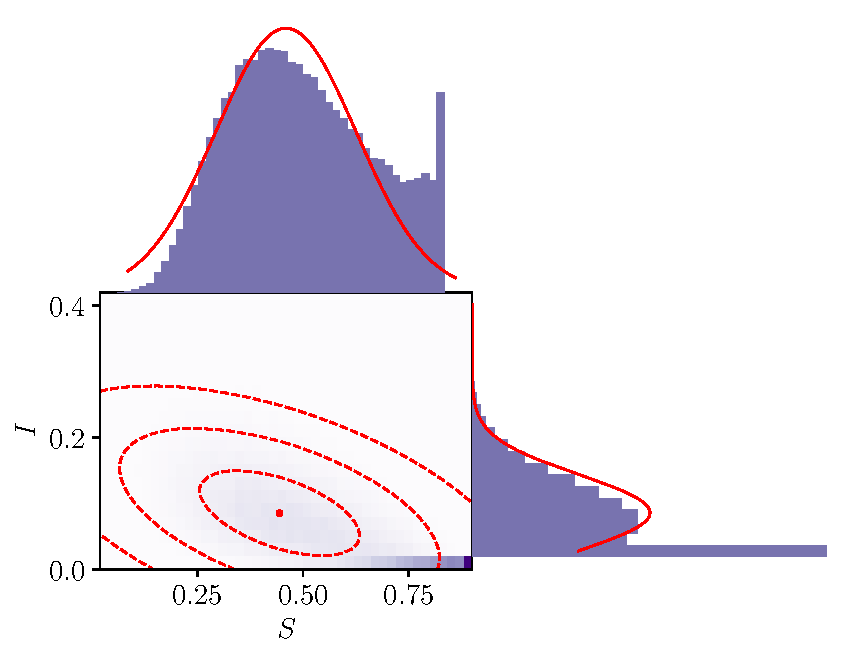
\includegraphics[width=\textwidth]{chp06_applications/figures/sir/sir_pairwise_50}
			\caption{\(M = 50\)}
			\label{fig:sir_gauss_rels_1}
		\end{subfigure}
		\begin{subfigure}{0.49\textwidth}
			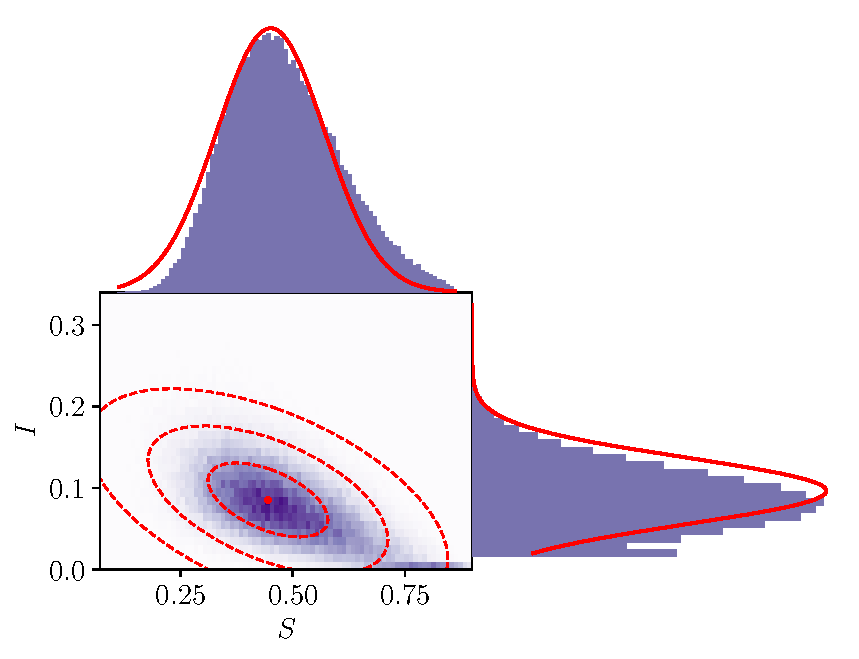
\includegraphics[width=\textwidth]{chp06_applications/figures/sir/sir_pairwise_100}
			\caption{\(M = 100\)}
			\label{fig:sir_gauss_rels_2}
		\end{subfigure}
		\begin{subfigure}{0.49\textwidth}
			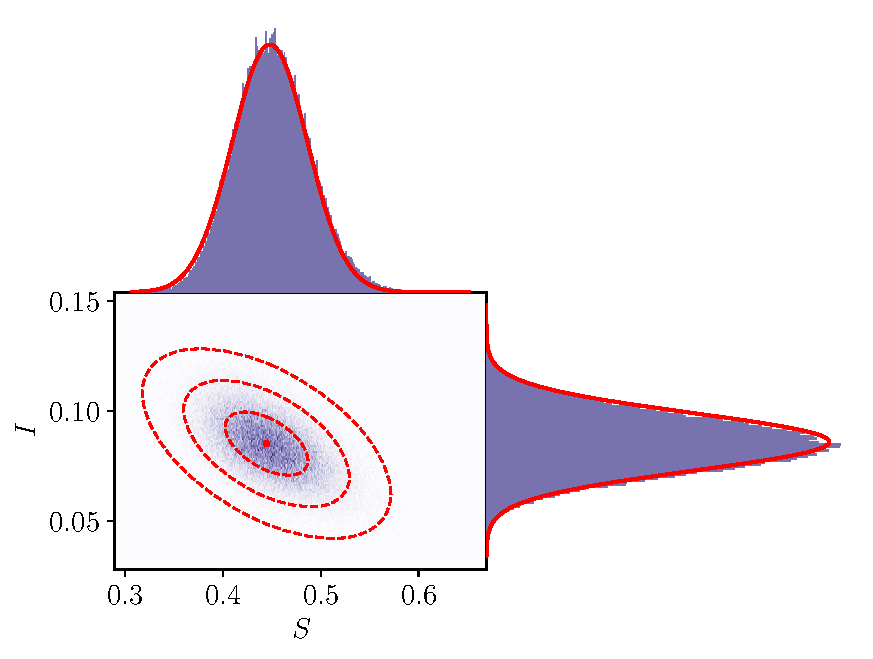
\includegraphics[width=\textwidth]{chp06_applications/figures/sir/sir_pairwise_1000}
			\caption{\(M = 1000\)}
			\label{fig:sir_gauss_rels_3}
		\end{subfigure}\begin{subfigure}{0.49\textwidth}
			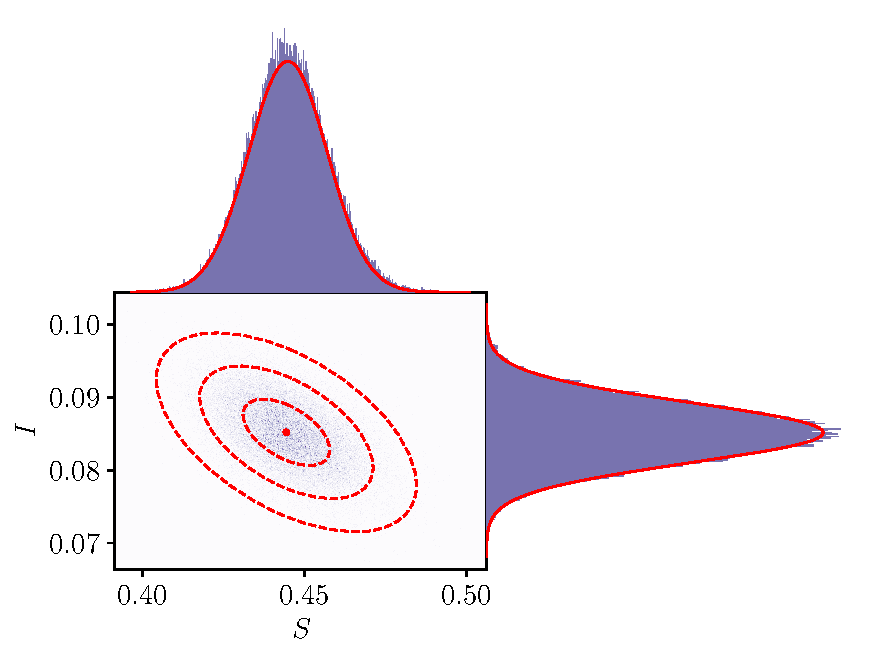
\includegraphics[width=\textwidth]{chp06_applications/figures/sir/sir_pairwise_10000}
			\caption{\(M = 10000\)}
			\label{fig:sir_gauss_rels_4}
		\end{subfigure}
		\caption{Histograms of Monte-Carlo simulations of the density process for the SIR model (with marginal plots on each axis), and the probability density function of the corresponding solution to the diffusion limit \cref{eqn:sir_diff_limit} plotted in red.
			Each sample path is initialised with 10\% of the population infected (i.e. \(x_0 = \left(0.1, 0.9\right)^{\T}\)).}
		\label{fig:sir_gauss_rels}
	\end{center}
\end{figure}

However, \Cref{fig:sir_gauss_rels} also highlights the limitations of using Gaussian approximations for certain types of stochastic processes.
An \(n\)-dimensional Gaussian random variable has support on the entirety of \(\R^n\); that is, for any non-empty subset of \(\R^n\), there is a non-zero probability of the variable taking a value in that set.
However, in many situations we can enforce (often from physical considerations) boundary conditions on the state variable.
In the SIR model, the \(I = 0\) and \(S = 0\) boundaries are \emph{absorbing}, in the sense that once the stochastic process reaches those states, it remains there indefinitely with probability \(1\).
We also saw another example of boundaries in the Gulf Stream example in \Cref{sec:appl_ocean}; the dataset only contained velocity
Boundary issues were avoided by ensuring that the evolution of the deterministic trajectory was sufficiently far from the boundaries and the scale of uncertainty small enough so that the probability of a stochastic trajectory nearing the boundary is negligible.
An absorbing boundary can be accounted for by setting both the drift and diffusivity in the stochastic differential equation to zero on the boundary.
However, such adjustments will often violate the requirements of smoothness in these terms set out in \Cref{hyp:smooth}.
More generally, one can stochastic differential equations with boundary conditions, and it can be shown that such SDEs do in fact have unique solutions; an introduction to the formal treatment of stochastic differential equations with boundary conditions is provided by \citet{Pilipenko_2014_IntroductionStochasticDifferential}.
However, the presence of boundary conditions is beyond the scope of this thesis and we will instead ensure that we choose initial conditions and values so that the impact of boundaries is negligible.


For large populations, the Gaussian diffusion limit is a well-used approximation that has been employed across many different modelling scenarios \citep[e.g.]{PollettEtAl_2010_ModellingPopulationProcesses}.
Rather, we are interested in the moderate-sized population case where the population is large enough to limit the practicality of Monte-Carlo simulation, but is small enough that the density process distributions demonstrate departures from Gaussianity.
Our aim is to employ the GMM algorithm to provide computationally efficient approximations in these scenarios, which we explore on a 5-dimensional example informed by real data in the next section (\Cref{sec:epi_5d}).

Next, we will compute the stochastic sensitivity field on the set of (physically relevant) initial conditions to the SIR model.



\begin{figure}
	\begin{center}
		\begin{subfigure}{0.49\textwidth}
			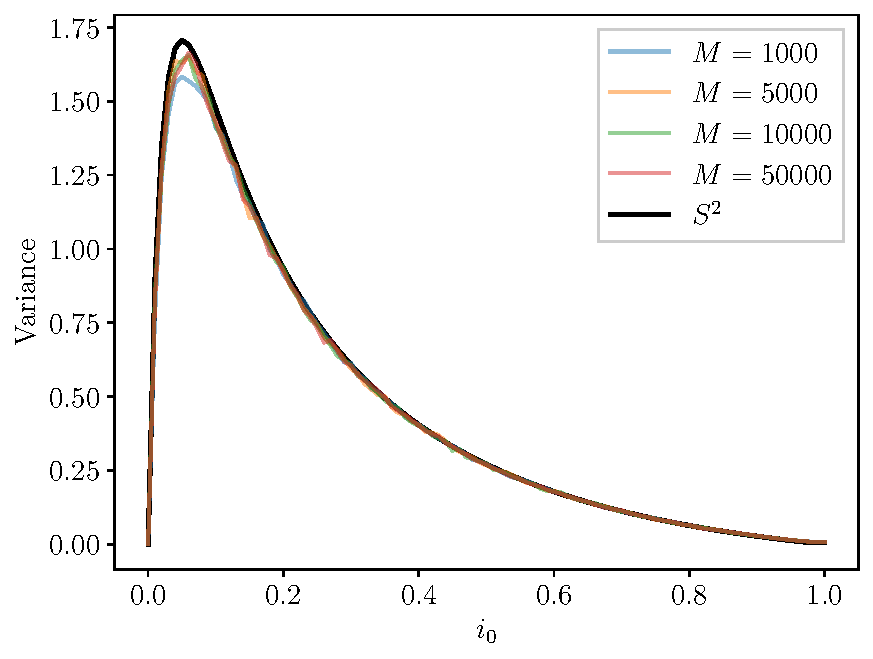
\includegraphics[width=\textwidth]{chp06_applications/figures/sir/sir_s2_1.0_1.0.pdf}
			\caption{\(\beta = 1\), \(\gamma = 1\) (\(R_0 = 1\))}
		\end{subfigure}
		\begin{subfigure}{0.49\textwidth}
			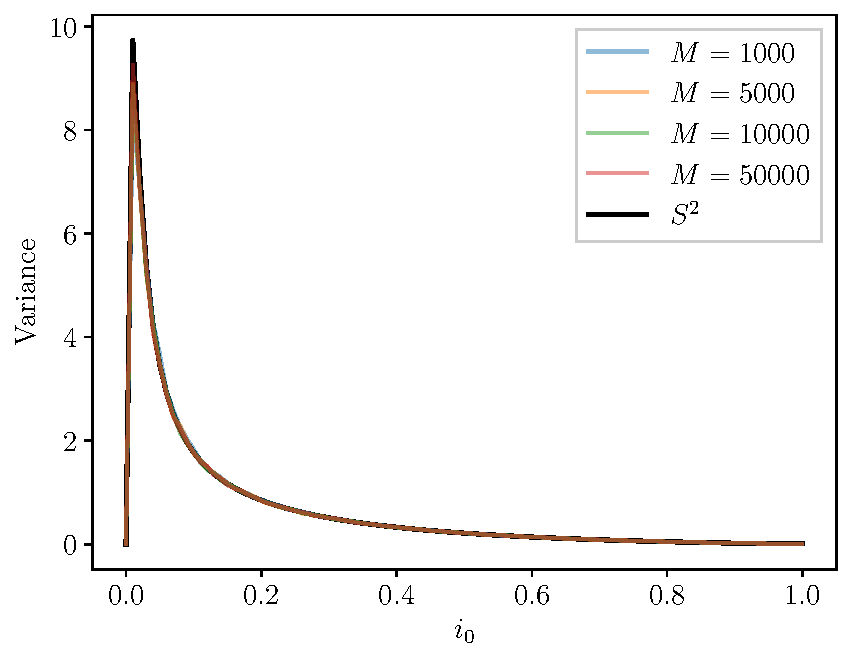
\includegraphics[width=\textwidth]{chp06_applications/figures/sir/sir_s2_1.5_1.0.pdf}
			\caption{\(\beta = 1.5\), \(\gamma = 1\) (\(R_0 = 1.5\))}
		\end{subfigure}\begin{subfigure}{0.49\textwidth}
			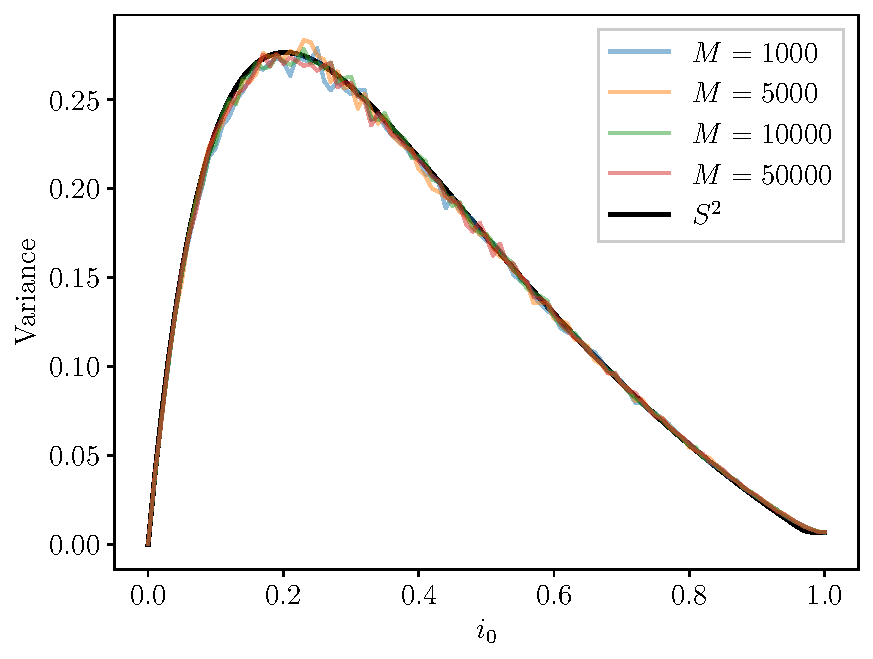
\includegraphics[width=\textwidth]{chp06_applications/figures/sir/sir_s2_0.5_1.0.pdf}
			\caption{\(\beta = 0.5\), \(\gamma = 1\) (\(R_0 = 0.5\))}
		\end{subfigure}
		% \begin{subfigure}{0.49\textwidth}
		% 			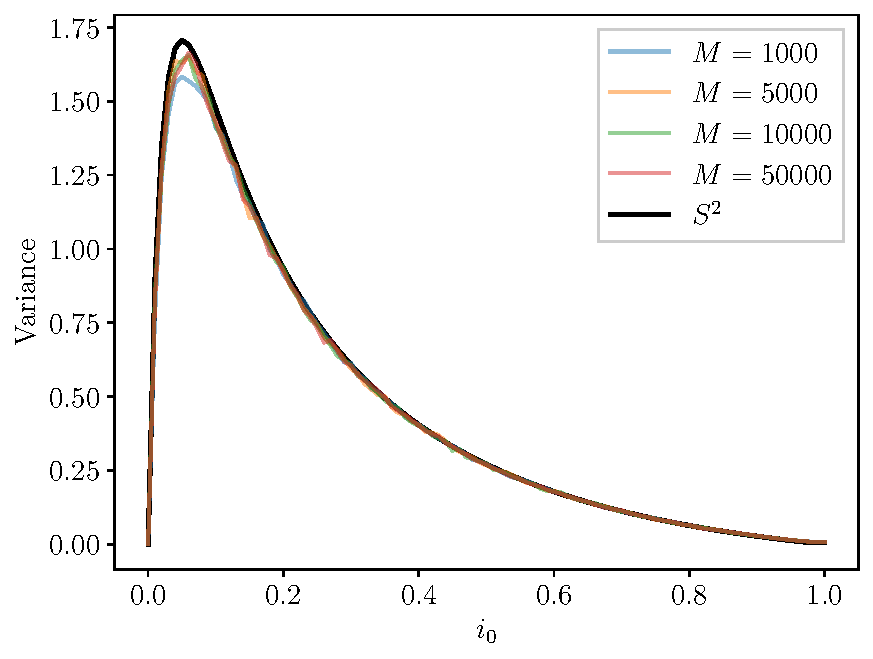
\includegraphics[width=\textwidth]{chp06_applications/figures/sir/sir_s2_1.0_1.0.pdf}
		% 			\caption{\(\beta = 2.0\), \(\gamma = 1\) (\(R_0 = 1\))}
		% 		\end{subfigure}
		\caption{The stochastic sensitivity value (in black) of the SIR diffusion limit \cref{eqn:sir_diff_limit} at time \(T = 5\), for varying initial condition \((1 - i_0, i_0)^{\T}\).
			The maximum projection of the sample covariance matrix (in various colours) for \(N = 10000\) stochastic simulations of the discrete population process over the same time interval is included.
			The corresponding initial condition is \(\left((1 - i_0)M, i_0 M\right)^{\T}\)}
		\label{fig:}
	\end{center}
\end{figure}






\subsection{Example 2: Household influenza model}\label{sec:epi_5d}


\begin{figure}
	\begin{center}
		\begin{tabular}{|c|c|c|c|}
			\hline
			Transition & \multicolumn{2}{c|}{Event}    & Rate \(\lambda_i\)                                                                                                     \\ \hline
			(1)        & Exposure                      & \(\left(S, E\right) \to \left(S-1, E+1\right)\)     & \(\left(\beta_I SI + \beta_H SH + \beta_F SF\right) / N\)        \\ \hline
			(2)        & Shedding                      & \(\left(E, I\right) \to \left(E - 1, I + 1\right)\) & \(\alpha E\)                                                     \\ \hline
			(3)        & Hospitalisation               & \(\left(I, H\right) \to \left(I - 1, H + 1\right)\) & \(\gamma_H \theta_1 I\)                                          \\ \hline
			(4)        & Hospital death without burial & \(\left(H, D\right) \to (H - 1, D + 1)\)            & \(\gamma_{dh}\delta_2 H\)                                        \\ \hline
			(5)        & Burial                        & \(\left(D\right) \to \left(D - 1\right)\)           & \(\gamma_f D\)                                                   \\ \hline
			(6)        & Death with burial             & \(\left(I\right) \to \left(I - 1\right)\)           & \(\gamma_i\left(1 - \theta_1\right)\left(1 - \delta_1\right) I\) \\ \hline
			(7)        & Death without burial          & \(\left(I, D\right) \to \left(I - 1, D + 1\right)\) & \(\delta_1 \left(1 - \theta_1\right) \gamma_d I\)                \\ \hline
			(8)        & Hospital death with burial    & \(\left(H\right) \to \left(H - 1\right)\)           & \(\gamma_{ih}\left(1 - \delta_2\right)H\)                        \\ \hline
		\end{tabular}

		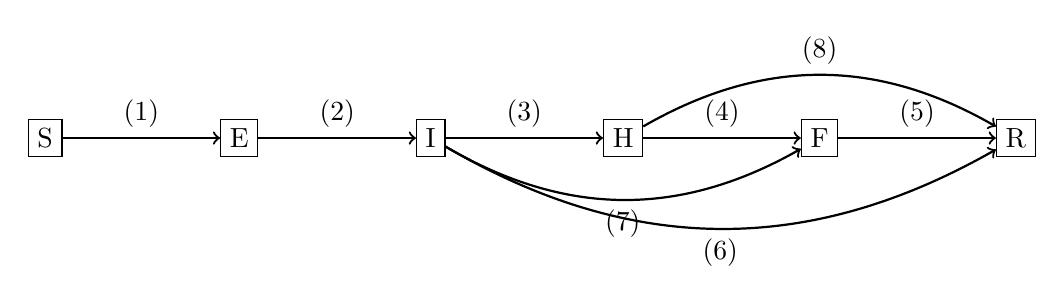
\begin{tikzpicture}
			\node (S) [draw] {S};
			\node (E) [draw, right=of S] {E};
			\node (I) [draw, right=of E] {I};
			\node (H) [draw, right=of I] {H};
			\node (F) [draw, right=of H] {F};
			\node (R) [draw, right=of F] {R};
			\path[->,thick] (S) edge[above] node{(1)}  (E)
			(E) edge[above] node{(2)} (I)
			(I) edge[above] node{(3)} (H)
			(H) edge[above] node{(4)} (F)
			(F) edge[above] node{(5)} (R)
			(I) edge[bend right, below] node{(6)} (R)
			(I) edge[bend right, below] node{(7)} (F)
			(H) edge[bend left, above] node{(8)} (R);
		\end{tikzpicture}
		\caption{Transition probabilities of the Ebola model.}
		\label{fig:ebola_transition}
	\end{center}
\end{figure}


The population process is also density dependent, with
\[
	f\!\left(\left(s, e, i, h, d\right), l\right) = \begin{cases}
		\beta_I s i + \beta_H sh + \beta_F sd,                        & \text{if } l = \left(-1, 1, 0, 0, 0\right), \\
		\alpha e,                                                     & \text{if } l = \left(0, -1, 1, 0, 0\right), \\
		\gamma_h \theta_1 i,                                          & \text{if } l = \left(0, 0, -1, 1, 0\right), \\
		\gamma_{dh}\delta_2 h,                                        & \text{if } l = \left(0, 0, 0, -1, 1\right), \\
		\gamma_f d,                                                   & \text{if } l = \left(0, 0, 0, 0, -1\right), \\
		\gamma_i\left(1 - \theta_1\right)\left(1 - \delta_1\right) i, & \text{if } l = \left(0,0,-1,0,0\right),     \\
		\delta_1\left(1 - \theta_1\right)\gamma_d i,                  & \text{if } l = \left(0,0,-1,0,1\right),     \\
		\gamma_{ih}\left(1 - \delta_2\right)h,                        & \text{if } l = \left(0,0,0,-1,0\right),     \\
		0,                                                            & \text{otherwise}.
	\end{cases}
\]
The deterministic differential equation is
\[
	\dod{X_t^{(\infty)}}{t} = \begin{bmatrix}
		-\beta_I X_t^{(\infty, 1)}X_t^{(\infty, 3)} - \beta_H X_t^{(\infty, 1)}X_t^{(\infty, 4)} - \beta_F X_t^{(\infty, 1)}X_t^{(\infty,5)}                                        \\
		\beta_I X_t^{(\infty, 1)}X_t^{(\infty, 3)} + \beta_H X_t^{(\infty, 1)}X_t^{(\infty, 4)} + \beta_F X_t^{(\infty, 1)}X_t^{(\infty,5)} - \alpha X_t^{(\infty, 2)}              \\
		\alpha X_t^{(\infty, 2)} - \left(\gamma_h + \gamma_i\left(1 - \theta_1\right)\left(1 - \delta_1\right) + \delta_1\left(1 - \theta_1\right)\gamma_d\right) X_t^{(\infty, 3)} \\
		\gamma_h\theta_1 X_t^{(\infty, 3)} - \gamma_{dh}\delta_2 X_t^{(\infty, 4)} - \gamma_{ih}\left(1 - \delta_2\right)X_t^{(\infty,4)}                                           \\
		\gamma_{dh}\delta_2 X_t^{(\infty, 4)} + \delta_1\left(1 - \theta_1\right)\gamma_d X_t^{(\infty, 3)} - \gamma_f X_t^{(\infty, 5)}
	\end{bmatrix}.
\]
